\documentclass[11pt,letterpaper]{report}

% ─── packages ────────────────────────────────────────────────────────────────
\usepackage[margin=1in]{geometry}
\usepackage[utf8]{inputenc}
\usepackage[T1]{fontenc}
\usepackage{lmodern}
\usepackage{microtype}
\usepackage{amsmath,amssymb,amsthm,bm}
\usepackage{mathtools}
\usepackage{graphicx}
\usepackage{float}
\usepackage{booktabs}
\usepackage{array}
\usepackage{longtable}
\usepackage{multirow}
\usepackage{caption}
\usepackage{subcaption}
\usepackage{xcolor}
\usepackage{listings}
\usepackage{tcolorbox}
\tcbuselibrary{listings,skins,breakable}
\usepackage{hyperref}
\usepackage{cleveref}
\usepackage{enumitem}

% ─── hyperref colors ─────────────────────────────────────────────────────────
\hypersetup{
  colorlinks=true,
  linkcolor=blue!60!black,
  citecolor=teal!60!black,
  urlcolor=magenta!60!black,
  pdftitle={SH-PPVI Handbook: Piecewise Potential Vorticity Inversion in Spherical Harmonics},
  pdfauthor={x\_yan},
}

% ─── code listings ───────────────────────────────────────────────────────────
\definecolor{codebg}{gray}{0.97}
\definecolor{codekw}{rgb}{0.13,0.29,0.53}
\definecolor{codestr}{rgb}{0.58,0.0,0.13}
\definecolor{codecom}{rgb}{0.25,0.50,0.25}
\lstdefinelanguage{Python}{
  keywords={def,class,import,from,as,return,if,elif,else,for,while,in,not,and,or,
           is,None,True,False,lambda,try,except,finally,raise,with,pass,break,continue,
           yield,global,nonlocal,assert,del},
  keywordstyle=\color{codekw}\bfseries,
  comment=[l]{\#},
  commentstyle=\color{codecom}\itshape,
  morestring=[b]",
  morestring=[b]',
  stringstyle=\color{codestr},
  sensitive=true,
}
\lstset{
  language=Python,
  basicstyle=\ttfamily\footnotesize,
  backgroundcolor=\color{codebg},
  frame=single,
  framerule=0pt,
  rulecolor=\color{codebg},
  showstringspaces=false,
  breaklines=true,
  numbers=left,
  numberstyle=\tiny\color{gray},
  xleftmargin=1.5em,
  framexleftmargin=1em,
}

% ─── math shorthands ─────────────────────────────────────────────────────────
\newcommand{\bpsi}{\bar{\psi}}
\newcommand{\bPhi}{\bar{\Phi}}
\newcommand{\bq}{\bar{q}}
\newcommand{\bu}{\bar{u}}
\newcommand{\bv}{\bar{v}}
\newcommand{\bzeta}{\bar{\zeta}}
\newcommand{\dpsi}{\delta\psi}
\newcommand{\dPhi}{\delta\Phi}
\newcommand{\dq}{q^{\prime}}
\newcommand{\dzeta}{\delta\zeta}
\newcommand{\du}{\delta u}
\newcommand{\dv}{\delta v}
\newcommand{\Lap}{\nabla^{2}}
\newcommand{\Lapinv}{\nabla^{-2}}
\newcommand{\R}{\mathbb{R}}
\newcommand{\PVU}{\,\mathrm{PVU}}
\newcommand{\Aavo}{A_{\mathrm{avo}}}
\newcommand{\Bstb}{B_{\mathrm{stb}}}
\DeclareMathOperator{\rmse}{RMSE}
\DeclareMathOperator{\corr}{corr}

% ─── theorem environments ────────────────────────────────────────────────────
\theoremstyle{definition}
\newtheorem{definition}{Definition}[chapter]
\newtheorem{proposition}{Proposition}[chapter]
\newtheorem{algorithm}{Algorithm}[chapter]

% ─── boxes ───────────────────────────────────────────────────────────────────
\newtcolorbox{keybox}[1][]{
  enhanced, breakable, colback=blue!4, colframe=blue!50!black,
  title=#1, fonttitle=\bfseries, sharp corners, boxrule=0.6pt,
}
\newtcolorbox{warnbox}[1][]{
  enhanced, breakable, colback=red!4, colframe=red!60!black,
  title=#1, fonttitle=\bfseries, sharp corners, boxrule=0.6pt,
}

% ─── title ───────────────────────────────────────────────────────────────────
\title{
  \vspace{-1cm}
  \Huge\bfseries Piecewise PV Inversion Handbook \\
  \LARGE The Wu Fortran Reference (Benchmark) \\
  \LARGE and the Python Spherical-Harmonic Port \\
  \vspace{0.5cm}
  \large \emph{For the 2025-01-08 California Blocking Case Study}
}
\author{
  \texttt{x\_yan} \\
  \small\texttt{pv\_inversion/}
}
\date{\today}

% ────────────────────────────────────────────────────────────────────────────
\begin{document}
\maketitle
\tableofcontents
\listoffigures
\listoftables

\chapter{Introduction and Overview}
\label{chap:intro}

\section{Purpose of this Handbook}

This handbook documents \textbf{piecewise potential-vorticity inversion}
(PPVI) for atmospheric blocking, as implemented in
\texttt{pv\_inversion/}.  The goal is to take the 2025-01-08 California
blocking event, partition its potential-vorticity (PV) anomaly into
vertical pieces, invert each piece to its own balanced circulation, and
thereby quantify how the upper-tropospheric PV anomaly, the
mid/low-tropospheric PV, and the \emph{surface thermal} anomaly each
contribute to the blocking flow.

The pipeline has a single numerical core: \textbf{W.~Wu's
finite-difference successive-over-relaxation (SOR) solver}
(\texttt{wu/fortran/pvpialln\_94UV.f}, \texttt{qinvert21\_94.f},
\texttt{qinvertp21\_94.f}), driven from a thin Python orchestration
layer (\texttt{wu/steps/}).  This Fortran is the same lineage as
C.~Davis's \texttt{PVPI.FOR} \cite{Davis1992} and the modern GFDL/CSU
PPVI tool; the inversion mathematics is unchanged, only the driving and
post-processing are in Python.

\begin{keybox}[What this handbook is about]
A \emph{single} working track --- the Wu Fortran pipeline --- on a
\textbf{nine-level} ERA5 grid, with the PV perturbation split into
\textbf{three pieces} that mirror the reference partition
$\{1\},\{2,3\},\{4..N_L\}$:
\begin{center}\small
\begin{tabular}{lll}
\toprule
piece & levels $K$ & physical content \\
\midrule
\textbf{surface} & $\{1\}$              & 1000\,hPa boundary $\theta$ (the surface heating) \\
\textbf{lower}   & $\{2,3\}$            & 850, 700\,hPa interior PV \\
\textbf{upper}   & $\{4,5,6,7,8,9\}$    & 500--200\,hPa interior PV $+$ 100\,hPa top $\theta$ \\
\bottomrule
\end{tabular}
\end{center}
The key conceptual point (\Cref{chap:math,chap:wu_solver}): the
\textbf{surface warm-$\theta$ anomaly is a boundary condition, not an
interior PV value} --- by Bretherton's equivalence it acts as a
PV \emph{sheet} at the lower boundary, and we invert it as its own
``surface'' piece.
\end{keybox}

\begin{warnbox}[Retired material]
Earlier drafts described a second ``Part~II'' spherical-harmonic (SH)
Python port and several Family-B solvers (a direct spectral solve and an
LGMRES/linearized-Charney solver).  \textbf{These have been removed.}
The SH BALNC/BALP port never converged and is no longer maintained;
this handbook documents only the Wu Fortran pipeline that runs
end-to-end.
\end{warnbox}

\section{The Case: 2025-01-08 California Block}

The event is a strong wintertime ridge over the northeast Pacific / west
coast of North America that contributed to the January 2025 California
wildfire outbreak.  At the analysis time (2025-01-08 00\,UTC) the
500\,hPa block centre is at $\approx 31.5^\circ$N, $222^\circ$E
($138^\circ$W), with $Z_{500}\approx 5890$\,m.  All cross-sections and
the 3-D structure figure (\Cref{sec:step11}) are centred on this point.

\section{Notation Cheat-Sheet}

\begin{center}
\begin{tabular}{ll}
  \toprule
  Symbol & Meaning \\
  \midrule
  $\psi$, $\Phi$ & streamfunction (m$^2$\,s$^{-1}$), geopotential (m$^2$\,s$^{-2}$) \\
  $\bpsi$, $\bPhi$ & climatological mean (basic) state \\
  $\dpsi=\psi-\bpsi$, $\dPhi=\Phi-\bPhi$ & anomalies \\
  $q$ & Ertel potential vorticity (PVU = $10^{-6}\,$K\,m$^2$\,kg$^{-1}$\,s$^{-1}$) \\
  $\bq$, $\dq=q-\bq$ & mean and anomalous PV \\
  $\theta_b$ & boundary potential temperature (surface / top) \\
  $\zeta=\Lap\psi$ & relative vorticity \\
  $f=2\Omega\sin\phi$, $f_0=f(45^\circ)$ & Coriolis parameter, reference value \\
  $\pi=(p/p_0)^{\kappa}$ & Exner function ($p_0=10^{5}$ Pa, $\kappa=R/c_p$) \\
  $\theta=T(p_0/p)^{\kappa}$ & potential temperature \\
  $K=1\ldots N_L$ & 1-indexed Fortran level ($K{=}1$ surface, $K{=}N_L$ top) \\
  $\Lap$, $\Lapinv$ & horizontal Laplacian and its inverse \\
  \bottomrule
\end{tabular}
\end{center}

A more complete glossary appears in \Cref{app:notation}.

\section{Quick Tour of the Code}

\begin{center}\small
\begin{tabular}{lll}
  \toprule
  Component & Purpose & Reference \\
  \midrule
  \texttt{config.py} / \texttt{wu/wu\_config.yaml} & grid, 9 levels, pieces, solver params & \Cref{chap:wu_solver} \\
  \texttt{wu/fortran/pvpialln\_94UV.f}  & Pass A/B: Ertel PV, $\bar\psi$, $\theta_b$ & \Cref{chap:wu_solver} \\
  \texttt{wu/fortran/qinvert21\_94.f}   & Pass C: total balanced inversion (BALNC) & \Cref{chap:wu_solver} \\
  \texttt{wu/fortran/qinvertp21\_94.f}  & Pass D: piecewise perturbation (BALP)    & \Cref{chap:wu_solver} \\
  \texttt{wu/steps/05\ldots11/}         & the step-by-step pipeline + plots         & \Cref{chap:wu_pipeline} \\
  \texttt{wu/steps/08/parse\_and\_pv.py} & Wu\,$Q\to$ SI Ertel PV ($\times10^{-8}$)  & \Cref{chap:wu_coeffs} \\
  \bottomrule
\end{tabular}
\end{center}

\noindent The shared front end (\texttt{shared\_steps/01\ldots04}) downloads
the ERA5 event hour, builds a 30-year climatology, and writes the
Fortran \texttt{.grid} input files; the Wu steps (05--11) compile and run
the four passes and produce all diagnostics.


\part{Theory and the Wu Fortran Reference (Benchmark)}
\chapter{Mathematical Foundations}
\label{chap:math}

\section{Coordinates and Constants}

The vertical coordinate is the \textbf{Exner pressure}
\begin{equation}
\boxed{\;\pi \equiv \left(\frac{p}{p_0}\right)^{\!\kappa}\;,\qquad
       p_0=10^{5}\,\mathrm{Pa},\qquad
       \kappa=\frac{R_d}{c_p}=\tfrac{2}{7}\approx 0.2857\;}
\label{eq:exner}
\end{equation}
with $\pi=1$ at the surface and $\pi\to 0$ at the model top.  The Wu
Fortran hardcodes $\kappa=2/7$ (this exact value is what makes the
$Q\to$\,SI conversion a clean constant, \Cref{chap:wu_coeffs}).  On the
$N_L=9$ ERA5 pressure levels used here,
\begin{equation}
\mathrm{PLEVS}=[1000,850,700,500,400,300,250,200,100]\ \mathrm{hPa},
\end{equation}
\begin{equation}
\pi_k = [\,1.000,\,0.955,\,0.903,\,0.820,\,0.770,\,0.709,\,0.673,\,0.631,\,0.518\,].
\end{equation}

\begin{center}\small
\begin{tabular}{lll}
  \toprule
  Constant & Symbol & Value \\
  \midrule
  Gravity (Fortran)      & $g$        & $9.81$ m\,s$^{-2}$ \\
  Dry-air gas constant   & $R_d$      & $287$ J\,kg$^{-1}$\,K$^{-1}$ \\
  Specific heat at $p$   & $c_p$      & $1004.5$ J\,kg$^{-1}$\,K$^{-1}$ (Fortran)\\
  $\kappa=R_d/c_p$       & $\kappa$   & $2/7 \approx 0.2857$ \\
  Earth's rotation       & $\Omega$   & $7.292\times10^{-5}$ rad\,s$^{-1}$ \\
  Earth radius (Wu)      & $a=2{\times}10^{7}/\pi$ & $6.366\times10^{6}$ m  \\
  Reference pressure     & $p_0$      & $10^{5}$ Pa \\
  Reference Coriolis     & $f_0$      & $f(45^\circ)\approx 1.031\times10^{-4}$ s$^{-1}$ \\
  \bottomrule
\end{tabular}
\end{center}

\section{Thermodynamic Relations}

\textbf{Potential temperature}
\begin{equation}
\theta = T\left(\frac{p_0}{p}\right)^{\!\kappa}.
\end{equation}
The Fortran is fed \emph{raw temperature} $T$ and forms $\theta$
internally as $\theta = T\,c_p/\Pi$ with $\Pi=c_p(p/p_0)^\kappa$
(\texttt{pvpialln\_94UV.f}); feeding it $\theta$ would double-convert and
inflate the static stability.

\textbf{Hydrostatic balance in Exner coordinates}
\begin{equation}
\boxed{\;\frac{\partial\Phi}{\partial\pi}=-c_p\,\theta\;}
\label{eq:hydrostatic}
\end{equation}
is the vertical link between $\Phi$ and $\theta$ that closes the
inversion and \emph{defines the boundary condition} of
\Cref{sec:boundary_theta}.

\section{Ertel Potential Vorticity}

The hydrostatic Ertel PV is
\begin{equation}
Q = -g(\zeta+f)\frac{\partial\theta}{\partial p}
    - g\Bigl(\frac{\partial u}{\partial p}\frac{\partial\theta}{\partial y}
            - \frac{\partial v}{\partial p}\frac{\partial\theta}{\partial x}\Bigr),
\label{eq:Q}
\end{equation}
in SI units K\,m$^2$\,kg$^{-1}$\,s$^{-1}$ ($\equiv 10^{-6}$\,PVU).  The
Wu Fortran evaluates an Exner-coordinate form of \cref{eq:Q}; its exact
relation to SI is derived in \Cref{chap:wu_coeffs}.

\begin{warnbox}[Interior PV exists only on the interior levels]
\texttt{pvpialln} computes $Q$ only on the \emph{interior} levels
$K=2\ldots N_L-1$ (850--200\,hPa): the vertical derivative
$\partial\theta/\partial\pi$ needs neighbours on both sides.  At the
surface ($K{=}1$, 1000\,hPa) and top ($K{=}N_L$, 100\,hPa) there is
\textbf{no interior PV} --- those two levels instead carry the
\emph{boundary potential temperature} of \Cref{sec:boundary_theta}.
This is why a surface-confined thermal anomaly shows ``no PV at
1000\,hPa'' in the interior field.
\end{warnbox}

\section{Boundary Potential Temperature as a PV Sheet}
\label{sec:boundary_theta}

The two boundary levels are represented by the half-level-averaged
potential temperature (\texttt{pvpialln\_94UV.f}, the lines that set
\texttt{THB,THT}):
\begin{equation}
\theta_b^{\text{(bot)}} = \tfrac12\bigl(\theta_{K=1}+\theta_{K=2}\bigr),\qquad
\theta_b^{\text{(top)}} = \tfrac12\bigl(\theta_{K=N_L-1}+\theta_{K=N_L}\bigr).
\end{equation}
In the \texttt{q.out} file the layout is therefore
$[\,\theta_b^{\text{bot}},\ \theta_b^{\text{top}},\ Q_{K=2},\ldots,Q_{K=N_L-1}\,]$
--- boundary $\theta$ first, interior PV after.

Through hydrostatic balance \cref{eq:hydrostatic}, $\theta_b$ specifies
the \emph{vertical derivative} of the geopotential / streamfunction at
the boundary, i.e.\ an \textbf{inhomogeneous Neumann boundary
condition}.  In \texttt{qinvert21\_94.f} (BALNC) it enters the elliptic
stencil one node inside each boundary (the lines that add
$+\theta_b^{\text{bot}}/\Delta\pi$ at $K{=}2$ and
$-\theta_b^{\text{top}}/\Delta\pi$ at $K{=}N_L-1$) and reconstructs the
boundary layer by a half-step hydrostatic integration,
$H_{1}=H_{2}+\theta_b^{\text{bot}}(\pi_2-\pi_1)$.  If no boundary
$\theta$ is supplied, the code applies \emph{homogeneous} Neumann
conditions.

\begin{keybox}[Bretherton: surface theta as a boundary PV sheet]
A warm surface potential-temperature anomaly is dynamically equivalent
to a \emph{positive} PV anomaly concentrated as a delta-function sheet
at the lower boundary; a cold anomaly $\equiv$ a negative sheet.  By the
PV--inversion (``invertibility'') principle this induces a circulation:
\[
\theta_b'>0\ (\text{warm}) \;\Rightarrow\; \text{cyclonic } \psi'\ (\psi'<0 \text{ in NH}),
\qquad
\theta_b'<0\ (\text{cold}) \;\Rightarrow\; \text{anticyclonic}.
\]
This is the textbook ``PV-thinking'' interpretation
\cite{HoskinsMcIntyreRobertson1985} of the Neumann condition above; the
Fortran implements the boundary condition, not the interpretation.  It
is the reason the \textbf{surface piece is inverted separately}
(its PV ``lives in'' the boundary $\theta$), and why for this event the
surface-piece $\psi'$ is predominantly cyclonic (the domain-mean surface
$\theta'$ is net warm, $\approx +1$\,K).
\end{keybox}

\section{Linearization and Balance Closure}
\label{sec:closure}

Decompose $\psi=\bpsi+\dpsi$, $\Phi=\bPhi+\dPhi$.  The piecewise solver
inverts the PV/boundary-$\theta$ \emph{perturbation}
$\dq=q_{\text{event}}-q_{\text{mean}}$ under a balance constraint.  The
production configuration uses the \textbf{nonlinear} balance
(\texttt{INLIN}=1, \Cref{sec:wu_params}): the operator coefficients are
evaluated about the half-state $\bar\cdot + \tfrac12(\cdot)'$
(\texttt{CNLIN}=0.5 in \texttt{qinvertp21\_94.f}), so that the three
piecewise solutions \emph{sum to the total} perturbation,
\begin{equation}
\boxed{\;\dpsi_{\text{surface}}+\dpsi_{\text{lower}}+\dpsi_{\text{upper}}
       \;\approx\;\dpsi_{\text{total}}\;}
\label{eq:additivity}
\end{equation}
to solver tolerance (the linear-closure check of \Cref{sec:step11}).

\begin{warnbox}[Why INLIN=1 rather than INLIN=0]
Earlier notes claimed \texttt{INLIN}=0 (linear balance) was
\emph{mandatory} because the nonlinear balance ``explodes at the jet.''
On the current 9-level, extended-domain configuration the
\textbf{nonlinear balance \texttt{INLIN}=1 converges} (all three pieces
reach \texttt{TOTAL CONVERGENCE}) and is required for the additivity
\cref{eq:additivity}.  \texttt{INLIN}=0 is no longer used.
\end{warnbox}

\chapter{The Wu Fortran Solver}
\label{chap:wu_solver}

This chapter describes the numerical core: W.~Wu's finite-difference
piecewise PV-inversion code, driven from Python (\texttt{wu/steps/})
while the solver itself remains the original Fortran-77.  The three
programs live in \texttt{wu/fortran/} and are compiled with
\texttt{gfortran -std=legacy -O2 -fno-automatic}.

\section{Grid and Vertical Levels}
\label{sec:wu_grid}

The solver runs on an extended Northern-Hemisphere window
(\texttt{config.py}, \texttt{wu/wu\_config.yaml}):

\begin{center}\small
\begin{tabular}{lll}
  \toprule
  Quantity & Symbol / code & Value \\
  \midrule
  Longitudes & $N_X$ & $134$ \\
  Latitudes  & $N_Y$ & $51$ \\
  Levels     & $N_W=N_L$ & $9$ \\
  Latitude row & $\phi_i = 85.5 - 1.5\,i$ & $85.5^\circ\!\to\!10.5^\circ$ (N$\to$S) \\
  Longitude col & $\lambda_j = 120 + 1.5\,j$ & $120^\circ\mathrm{E}\!\to\!319.5^\circ\mathrm{E}$ ($=40.5^\circ$W) \\
  Pressure levels & PLEVS [hPa] & $1000,850,700,500,400,$ \\
                  &             & $300,250,200,100$ \\
  Earth radius & $a=2\times10^{7}/\pi$ & $6.366\times10^{6}$ m \\
  Grid spacing & $\Delta p=\Delta l = a\,\mathrm{rad}(1.5^\circ)$ & $1.667\times10^{5}$ m \\
  \bottomrule
\end{tabular}
\end{center}

\begin{warnbox}[Fortran \texttt{PARAMETER} blocks are hard-wired]
$N_X,N_Y,N_W$ appear as compile-time \texttt{PARAMETER}s inside
\emph{every} \texttt{.f} file (and inside each subroutine).  Changing the
grid requires editing and recompiling the Fortran --- not just
\texttt{config.py}.  The current 9-level build sets \texttt{NW=9},
\texttt{NL=9}, and a 9-value \texttt{DATA PR} array in all three sources.
The Python drivers pass solver \emph{parameters} (relaxation factors,
piece definitions) over \texttt{stdin}; they cannot change array
dimensions.
\end{warnbox}

\section{The Three Programs and Four Passes}
\label{sec:wu_passes}

\begin{center}\small
\begin{tabular}{llll}
  \toprule
  Pass & Program & Subroutine & Produces \\
  \midrule
  A & \texttt{pvpialln}  & ---    & \texttt{meanq}, \texttt{meanh} (mean $Q$, $\theta_b$, $\psi$) \\
  B & \texttt{pvpialln}  & ---    & \texttt{event\_q.out}, \texttt{event\_h.out} \\
  C & \texttt{qinvert21} & BALNC  & \texttt{event\_bal.out} (total balanced $\psi$, $\Phi$) \\
  D & \texttt{qinvertp21}& BALP   & \texttt{event\_pert.out} (3-piece $\psi'$) \\
  \bottomrule
\end{tabular}
\end{center}

\paragraph{Pass A/B --- \texttt{pvpialln}.}  Computes the boundary
potential temperatures $\theta_b^{\text{bot}},\theta_b^{\text{top}}$
(\Cref{sec:boundary_theta}), the Ertel-like PV on the interior levels
($K=2\ldots N_W{-}1$, i.e.\ 850--200\,hPa), the balanced streamfunction
$\psi$ from relative-vorticity inversion, and the geopotential.  Pass~A
runs on the 30-year climatological mean state; Pass~B on the
2025-01-08 event state.  The \texttt{q.out} layout is
$[\theta_b^{\text{bot}},\theta_b^{\text{top}},Q(K{=}2..N_W{-}1)]$.

\paragraph{Pass C --- \texttt{qinvert21} (BALNC).}  The full
\emph{total} balanced inversion: a 2-D Helmholtz problem for $\psi$ on
each level coupled to a 3-D PV--$\psi$ relation under gradient-wind
balance, by SOR with under-relaxation between $\psi$ and $\Phi$.  The
boundary $\theta$ enters as the inhomogeneous Neumann condition of
\Cref{sec:boundary_theta}.

\paragraph{Pass D --- \texttt{qinvertp21} (BALP).}  Partitions the PV
\emph{perturbation} $\dq=q_{\text{event}}-q_{\text{mean}}$ into three
pieces and inverts each independently to its perturbation streamfunction
$\psi'$.  In the BALP convention a piece is a list \texttt{QLV} of level
indices, where the value \texttt{1} activates the \emph{lower-boundary}
$\theta$, \texttt{NL} the \emph{upper-boundary} $\theta$, and
$2..N_L{-}1$ the interior PV at that level:

\begin{center}\small
\begin{tabular}{llll}
  \toprule
  Piece & \texttt{QLV} & Activates & Pressures \\
  \midrule
  \textbf{surface} & $\{1\}$              & 1000\,hPa boundary $\theta$ only & --- \\
  \textbf{lower}   & $\{2,3\}$            & interior PV & $850,700$ hPa \\
  \textbf{upper}   & $\{4,5,6,7,8,9\}$    & interior PV $+$ top $\theta$ ($\texttt{9}{=}N_L$) & $500$--$200$ hPa $+\,100\,\theta$ \\
  \bottomrule
\end{tabular}
\end{center}

The three \texttt{QLV} lists cover every field
($\theta_b^{\text{bot}}$, interior PV at $K{=}2..8$, $\theta_b^{\text{top}}$)
exactly once, which is the precondition for the additivity
\cref{eq:additivity}.  The stdin actually sent is
\texttt{1,1}\,/\,\texttt{2,2,3}\,/\,\texttt{5,4,5,6,7,8,9}.

\begin{keybox}[The surface piece is the surface heating]
Because \texttt{QLV}=$\{1\}$ activates only the lower-boundary $\theta$,
the \textbf{surface piece is the inversion of the surface
warm/cold-$\theta$ anomaly} (the Bretherton PV sheet,
\Cref{sec:boundary_theta}) --- not of any interior 1000\,hPa PV (there is
none).  This isolates the surface thermal forcing from the
free-tropospheric PV, mirroring the reference inv3d partition.
\end{keybox}

\section{Solver Parameters}
\label{sec:wu_params}

Parameters are passed over \texttt{stdin} from \texttt{wu\_config.yaml}:

\begin{center}\small
\begin{tabular}{llll}
  \toprule
  Param & Pass C & Pass D & Role \\
  \midrule
  \texttt{OMEGS} & $1.4$  & $1.85$ & SOR factor, $\psi$ sweep \\
  \texttt{OMEGH} & $1.4$  & $1.4$  & SOR factor, $\Phi/H$ sweep \\
  \texttt{PART}  & $0.05$ & $0.05$ & under-relaxation $\psi\!\leftrightarrow\!\Phi$ \\
  \texttt{THRSH} & $0.01$ & $0.1$  & convergence threshold \\
  \texttt{INLIN} & ---    & $1$    & \textbf{nonlinear} balance (additivity) \\
  \texttt{IBC}   & ---    & $0$    & homogeneous Dirichlet lateral walls \\
  \bottomrule
\end{tabular}
\end{center}

\noindent \texttt{qinvertp21\_94.f} \emph{hardcodes} its iteration caps
and PV floor ($\texttt{MAX}=8000$, $\texttt{MAXT}=2000$,
$\texttt{QMIN}=10^{-5}$); the YAML does not set them.  The
non-dimensional Exner increment is $\texttt{DPI}=500/N_L=55.56$
(auto-scaled with $N_L$).

\section{Convergence and Closure (current behaviour)}
\label{sec:wu_converge}

\begin{itemize}\setlength\itemsep{2pt}
  \item \textbf{Pass D} converges cleanly: all three pieces report
        \texttt{TOTAL CONVERGENCE}, no NaNs, with physical magnitudes
        (the upper piece dominates the 250\,hPa response).
  \item \textbf{Pass C} prints \texttt{PHI CONVERGED} (per-cycle residual
        $\sim 10^{-4}$, below threshold) and then a \emph{benign}
        ``started diverging'' from \texttt{qinvert21}'s outer-coupling
        heuristic (it fires when an outer cycle needs $>\!10$ more inner
        iterations after $>\!30$ cycles).  The written
        \texttt{event\_bal.out} is the per-cycle-converged field
        (identical at $\omega=1.2$ and $1.4$); it is used as the total
        reference for Pass~D.
  \item \textbf{Top boundary 100\,hPa is non-uniform} ($\Delta\sigma$
        jumps $0.05\!\to\!0.10$ from 200 to 100\,hPa).  This is accepted:
        the 9-level grid closes the piecewise sum substantially better
        (linear-closure $R^2\!\approx\!0.44$ at 250\,hPa) than a
        uniform-top 8-level grid ($R^2\!\approx\!-0.2$), and all
        analysis of interest is at $\le 200$\,hPa.
\end{itemize}

\chapter{The Wu Pipeline, Step by Step}
\label{chap:wu_pipeline}

This chapter walks through the executable steps in \texttt{wu/steps/}
that take the raw Fortran output to the piecewise diagnostics.  Each
step is illustrated with the figure it generates (regenerated for this
handbook into \texttt{handbook/figs/wu/}).

\section{Step 05 --- Pass A/B: PV, Boundary \texorpdfstring{$\theta$}{theta}, Balanced \texorpdfstring{$\psi$}{psi}}
\label{sec:step05}

Step~05 compiles the three Fortran programs and runs \texttt{pvpialln}
twice: Pass~A on the 30-year mean state (\texttt{meanq}, \texttt{meanh})
and Pass~B on the 2025-01-08 event state (\texttt{event\_q.out},
\texttt{event\_h.out}).  It computes the boundary $\theta$
($\theta_b^{\text{bot}}$ at 1000, $\theta_b^{\text{top}}$ at 100\,hPa),
the interior Ertel PV on $850$--$200$\,hPa, and the balanced
streamfunction.

\begin{figure}[H]
  \centering
  
\includegraphics[width=\textwidth]{figs/wu/wu_mean_pv_3levels.png}
  \caption[Pass A mean Ertel PV]{\textbf{Step 05 / Pass A.} Mean-state
  Ertel PV (Wu internal units) at three representative \emph{interior}
  levels.  The upper-level panel shows the climatological jet PV gradient
  that the event anomaly perturbs.}
  \label{fig:wu_mean_pv}
\end{figure}

\begin{figure}[H]
  \centering
  
\includegraphics[width=\textwidth]{figs/wu/wu_pv_anomaly_3levels.png}
  \caption[Event PV anomaly]{\textbf{Step 05 / Pass B.} Event-minus-mean
  PV anomaly $\dq$.  The dominant upper-tropospheric positive anomaly is
  the blocking ridge inverted in the \emph{upper} piece of Pass~D; the
  weak low-level anomaly is dwarfed by it (and the surface heating itself
  lives in the boundary $\theta$, not in this interior field).}
  \label{fig:wu_pv_anom}
\end{figure}

\begin{figure}[H]
  \centering
  
\includegraphics[width=0.78\textwidth]{figs/wu/wu_mean_psi_500hpa.png}
  \caption[Balanced mean streamfunction]{\textbf{Step 05.} Balanced
  mean-state streamfunction $\bpsi$ at $500$\,hPa --- the basic state
  about which the nonlinear (\texttt{INLIN}=1) perturbation inversion is
  linearised.}
  \label{fig:wu_mean_psi}
\end{figure}

\section{Step 06 --- Pass C: Total Balanced Inversion (BALNC)}
\label{sec:step06}

Step~06 runs \texttt{qinvert21} (BALNC) to produce the total balanced
$(\psi,\Phi)$ pair (\texttt{event\_bal.out}), the reference from which
Pass~D forms the perturbation.  Per-cycle convergence is reached
($\sim 10^{-4}$, below threshold); the trailing ``started diverging''
message is the benign outer-coupling heuristic of
\Cref{sec:wu_converge}, and the written field is the converged state.

\begin{figure}[H]
  \centering
  
\includegraphics[width=\textwidth]{figs/wu/pass_c_psi_all_levels.png}
  \caption[Pass C all levels]{\textbf{Step 06 / Pass C.} Total balanced
  streamfunction at all nine pressure levels, showing the
  equivalent-barotropic vertical structure of the blocking circulation.}
  \label{fig:wu_passc_all}
\end{figure}

\section{Step 07 --- Pass D: Piecewise Perturbation Inversion (BALP)}
\label{sec:step07}

Step~07 runs \texttt{qinvertp21} (BALP), partitioning $\dq$ into the
\textbf{surface}, \textbf{lower} and \textbf{upper} pieces
(\Cref{sec:wu_passes}) and inverting each to its perturbation
streamfunction $\psi'$.  All three report \texttt{TOTAL CONVERGENCE}.

\begin{figure}[H]
  \centering
  
\includegraphics[width=\textwidth]{figs/wu/pass_d_psi_3pieces_250hpa.png}
  \caption[Pass D three pieces]{\textbf{Step 07 / Pass D.} $250$\,hPa
  perturbation streamfunction $\psi'$ induced by each piece:
  \textbf{(a)} surface ($1000$\,hPa boundary $\theta$),
  \textbf{(b)} lower ($850$--$700$\,hPa PV),
  \textbf{(c)} upper ($500$--$200$\,hPa PV $+$ $100$\,hPa top $\theta$).
  The upper piece dominates the jet-level response; the surface piece is
  a broad, predominantly cyclonic ($\psi'<0$) response to the net-warm
  surface $\theta'$.}
  \label{fig:wu_passd_3}
\end{figure}

\section{Step 08 --- Wu \texorpdfstring{$Q$}{Q} vs ERA5 Ertel PV}
\label{sec:step08}

Step~08 parses all Fortran outputs, converts Wu $Q$ to SI by the exact
$10^{-8}$ constant (\Cref{chap:wu_coeffs}), and computes the induced
winds and PV advection, writing \texttt{piecewise\_psi.nc} and
\texttt{pv\_advection.nc} (all SI).

\begin{figure}[H]
  \centering
  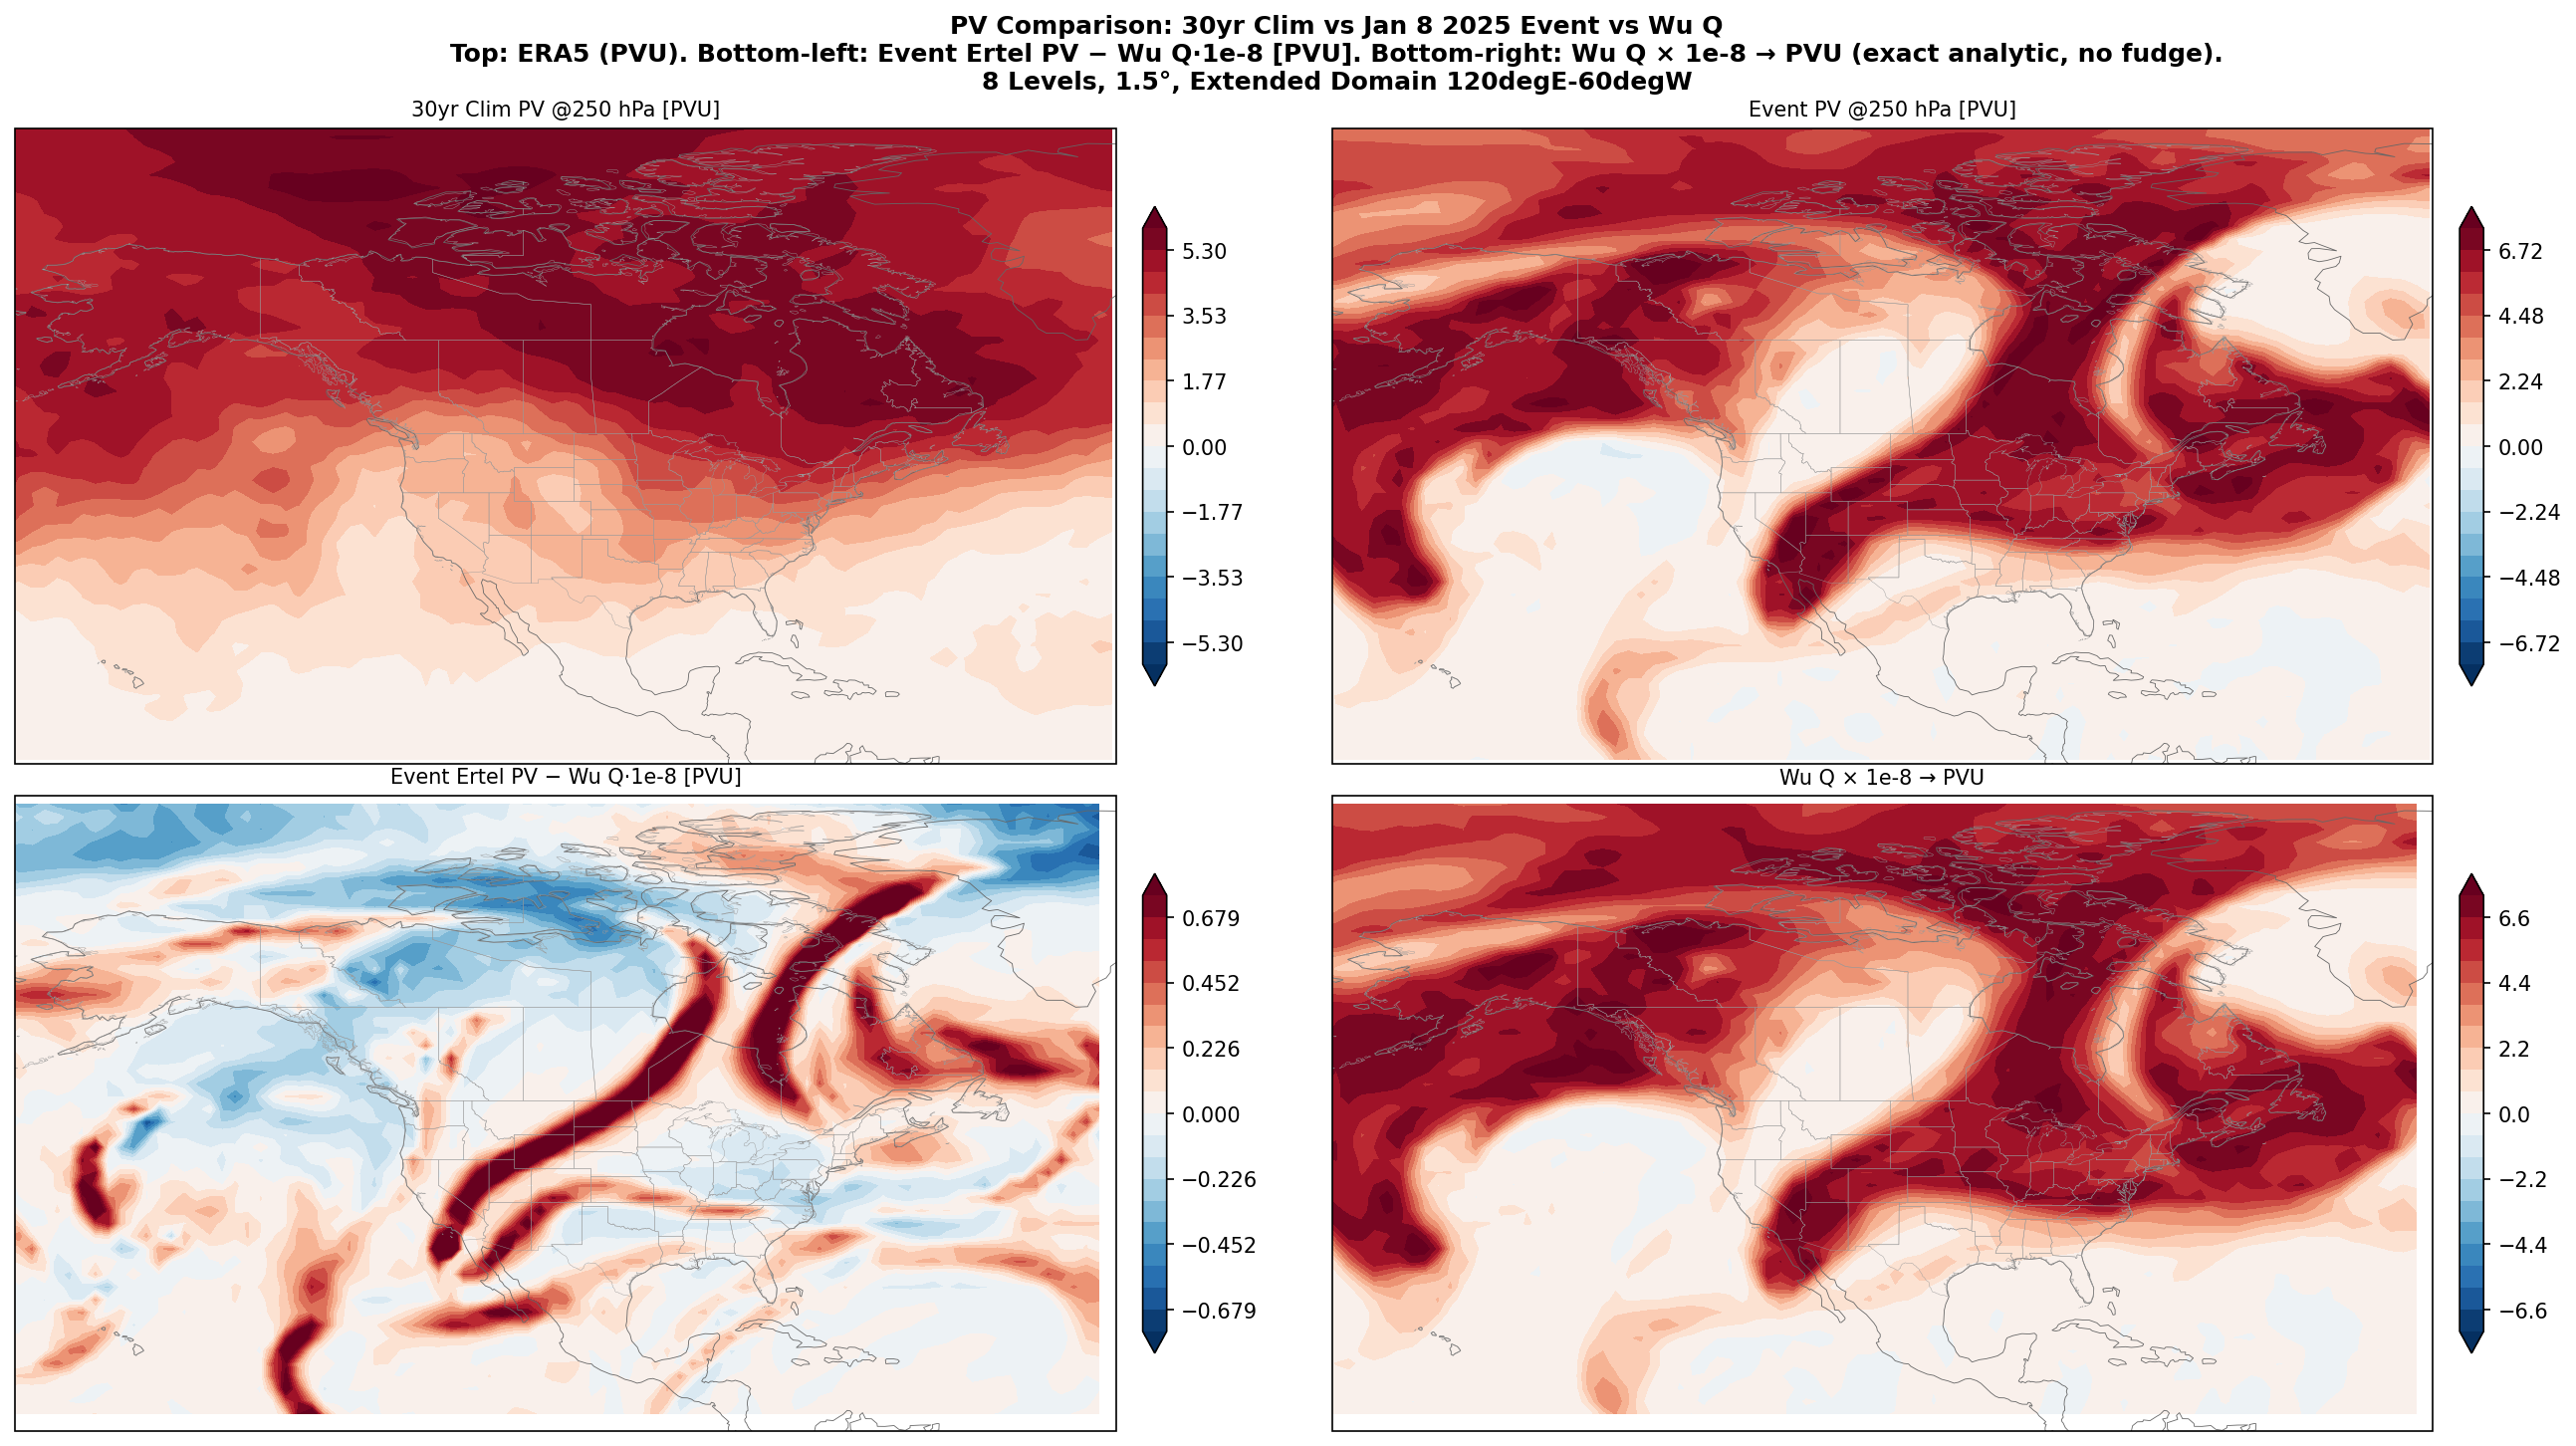
\includegraphics[width=0.85\textwidth]{figs/wu/pv_comparison_250hPa.png}
  \caption[Wu vs ERA5 PV]{\textbf{Step 08.} Wu $Q\times10^{-8}$ versus
  ERA5 native Ertel PV at $250$\,hPa.  After the raw-$T$ fix the median
  ratio is $1.00$ ($\corr=0.995$); no empirical scaling is used.}
  \label{fig:wu_vs_era5}
\end{figure}

\section{Step 10 --- Fig.~8 Replica (PV Advection)}
\label{sec:step10}

\begin{figure}[H]
  \centering
  
\includegraphics[width=0.92\textwidth]{figs/wu/fig8_replica.png}
  \caption[Davis 2022 Fig.~8 replica]{\textbf{Step 10.} Three-panel
  Davis-style PV-advection diagnostic, one panel per piece (surface /
  lower / upper): $250$\,hPa PV advection by the induced winds (fill),
  total PV anomaly (contours) and induced wind vectors (arrows).}
  \label{fig:wu_fig8}
\end{figure}

\section{Step 11 --- Cross-Sections and 3-D Structure}
\label{sec:step11}

Step~11 produces the latitude/longitude--pressure cross-sections and a
3-D ``vertical structure'' view, plus the linear-closure check.

\begin{figure}[H]
  \centering
  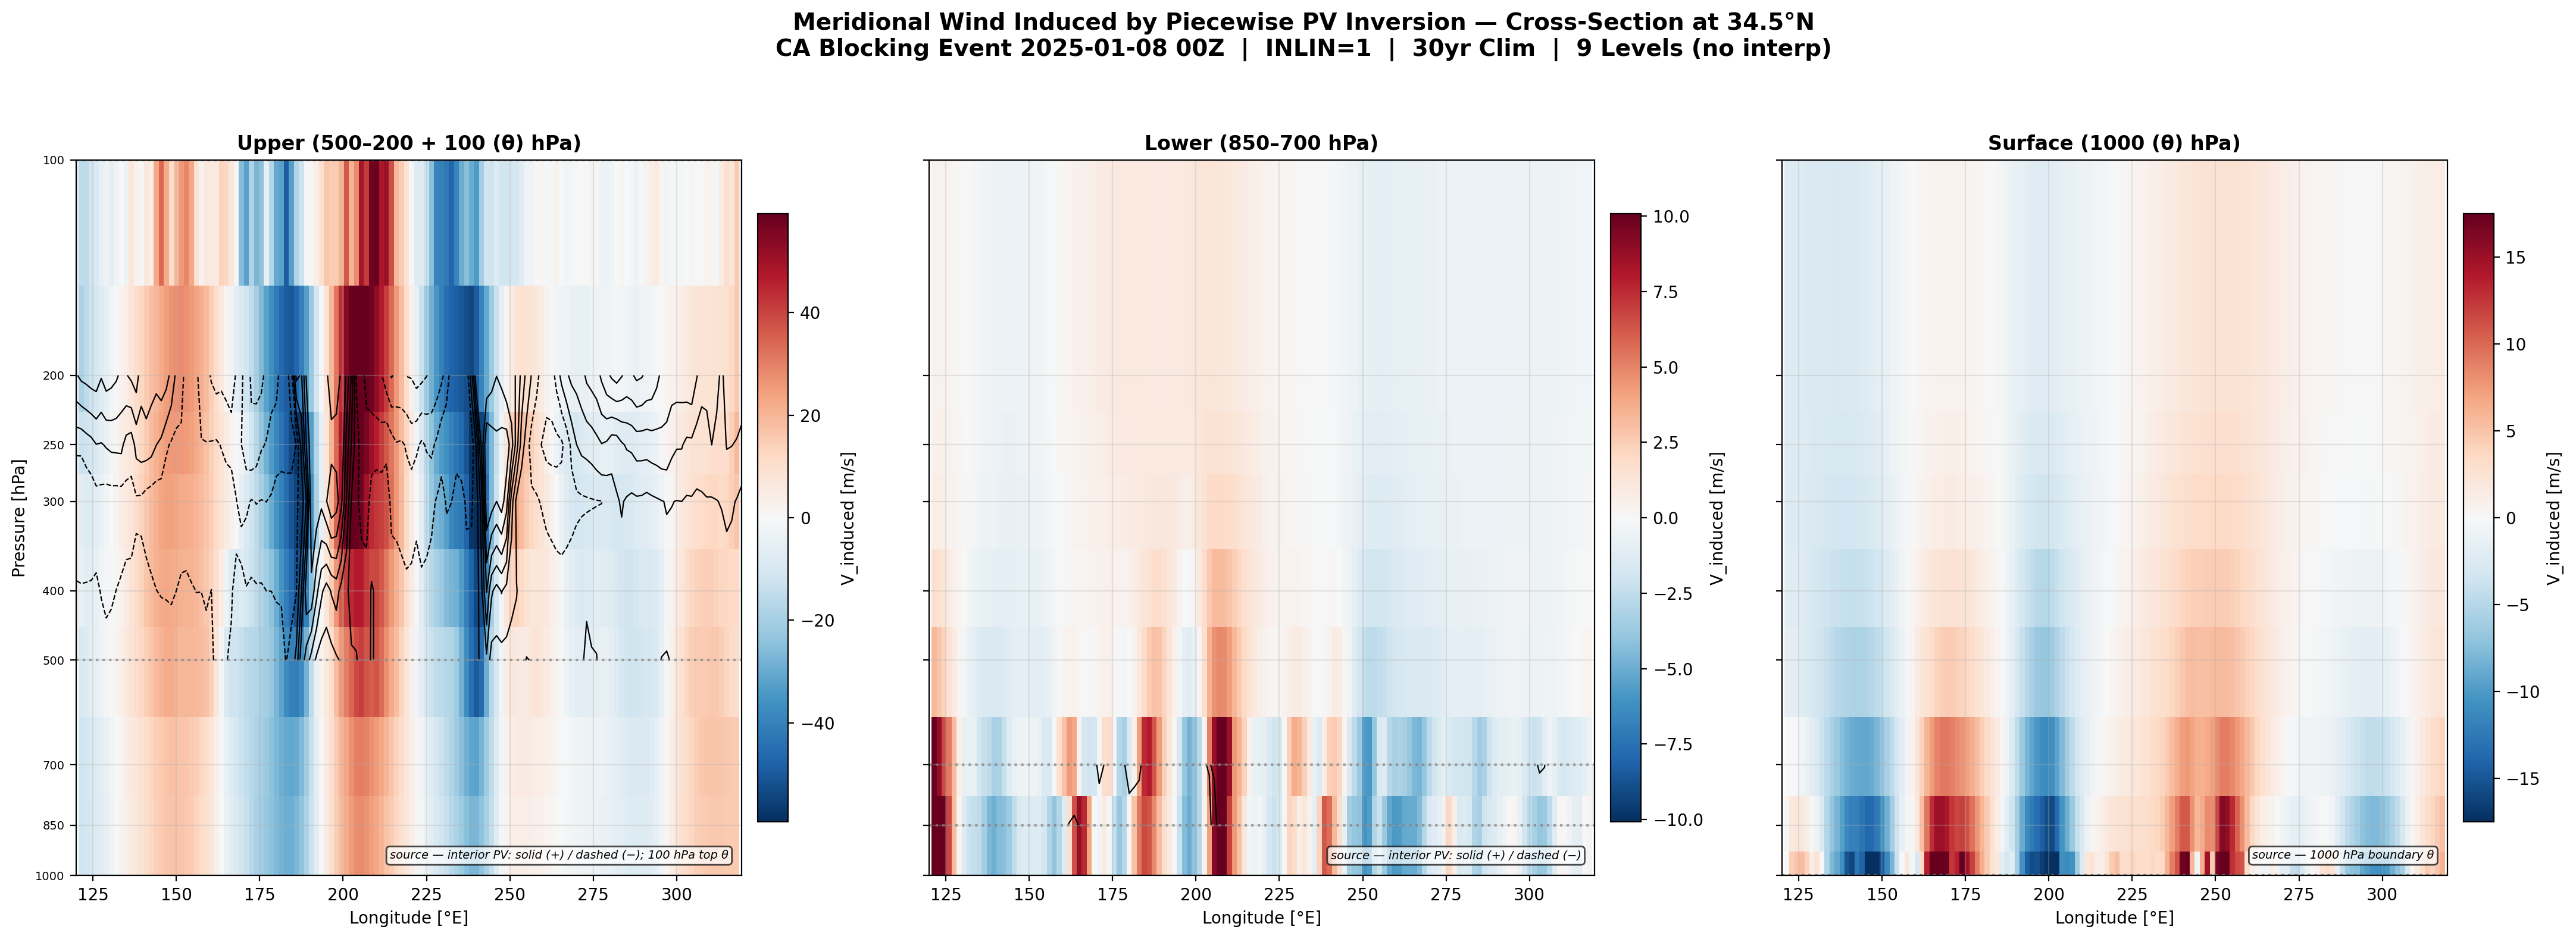
\includegraphics[width=\textwidth]{figs/wu/xsection_vinduced_3panel.png}
  \caption[Induced-wind cross-section]{\textbf{Step 11.} Zonal--vertical
  cross-section at $34.5^\circ$N of the meridional wind $v'$ induced by
  each piece, with each piece's \emph{own} source overlaid (interior PV
  contours; boundary-$\theta$ pieces labelled).  The \textbf{upper} piece
  peaks aloft ($\sim$250\,hPa, $\pm$50\,m\,s$^{-1}$); the \textbf{surface}
  piece is surface-trapped (peaks at 1000\,hPa, decaying upward) ---
  exactly the Bretherton boundary response.}
  \label{fig:wu_xsec}
\end{figure}

\begin{figure}[H]
  \centering
  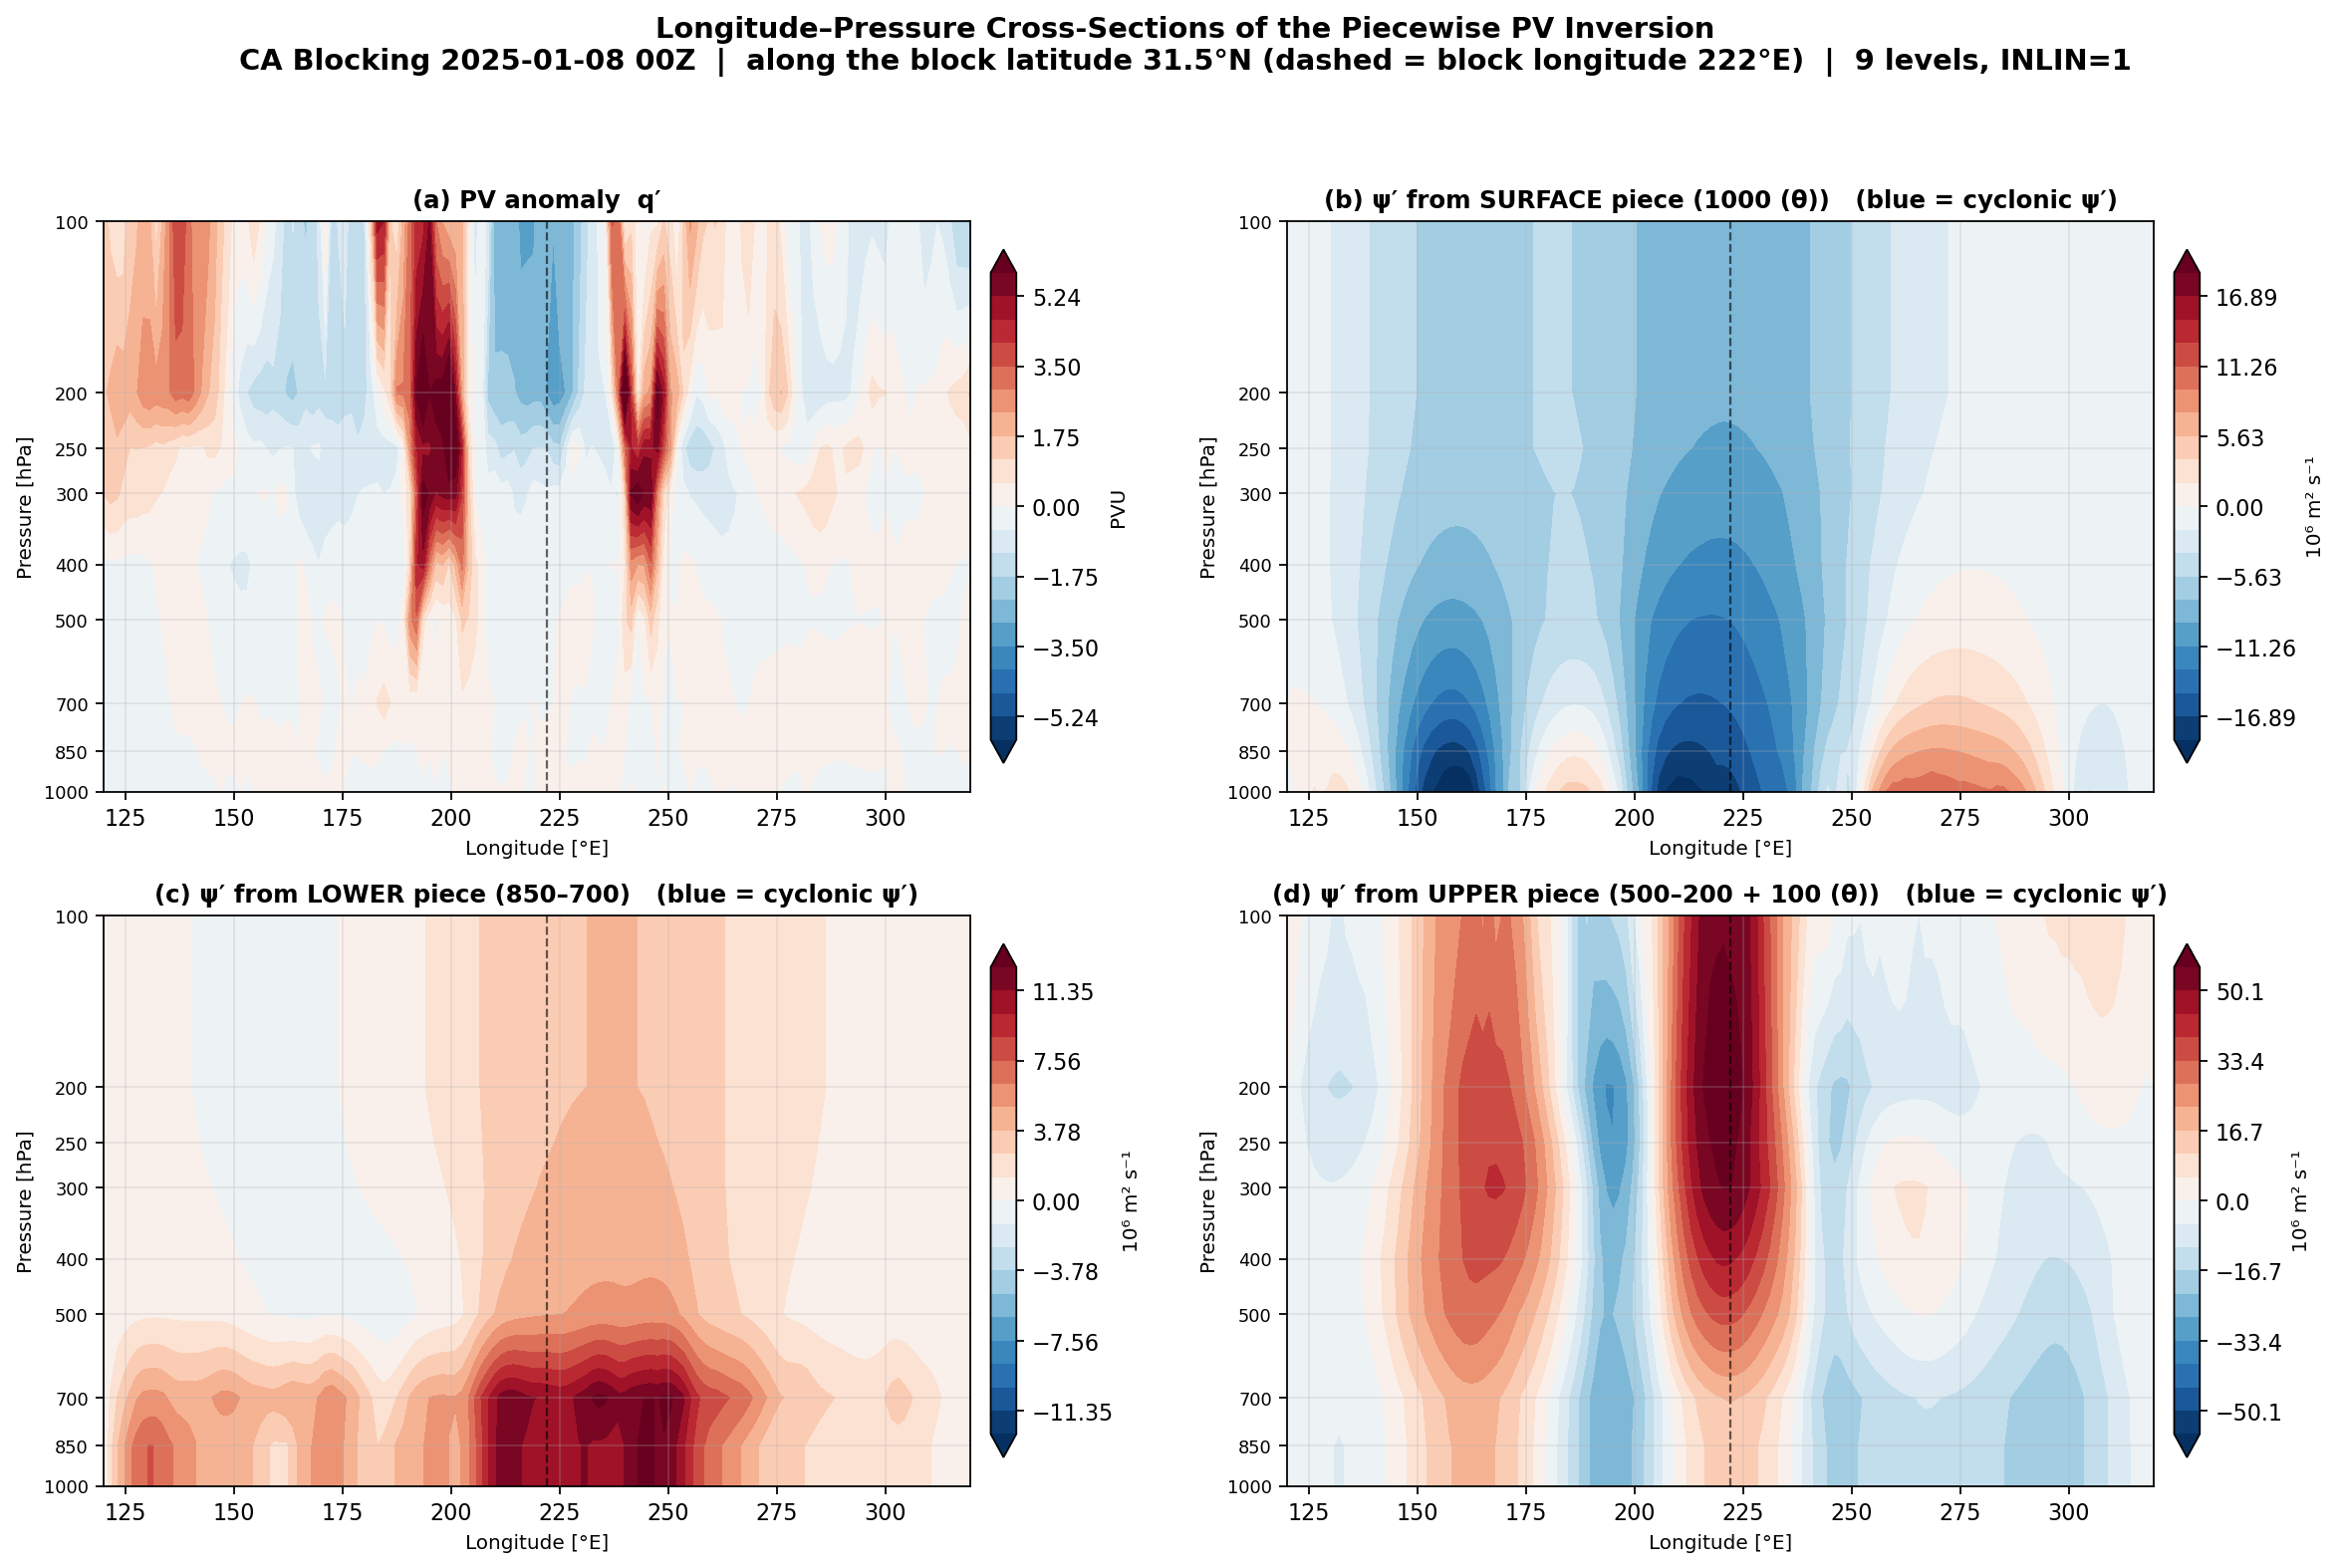
\includegraphics[width=\textwidth]{figs/wu/xsection_pv_psi_4panel.png}
  \caption[PV and piece-$\psi'$ cross-sections]{\textbf{Step 11.}
  Longitude--pressure ($x$--$p$) cross-sections at the block latitude
  ($31.5^\circ$N; dashed line $=$ block longitude $222^\circ$E):
  \textbf{(a)} total PV anomaly $q'$; \textbf{(b--d)} $\psi'$ induced by
  the surface, lower and upper pieces (blue $=$ cyclonic $\psi'<0$).  The
  PV anomaly is concentrated at upper levels (panel a); the surface
  boundary level carries no interior PV --- the surface heating is the
  boundary $\theta$ inverted in panel (b), a broad predominantly cyclonic
  response.  The upper piece (d) dominates the amplitude.}
  \label{fig:wu_3d}
\end{figure}

\begin{figure}[H]
  \centering
  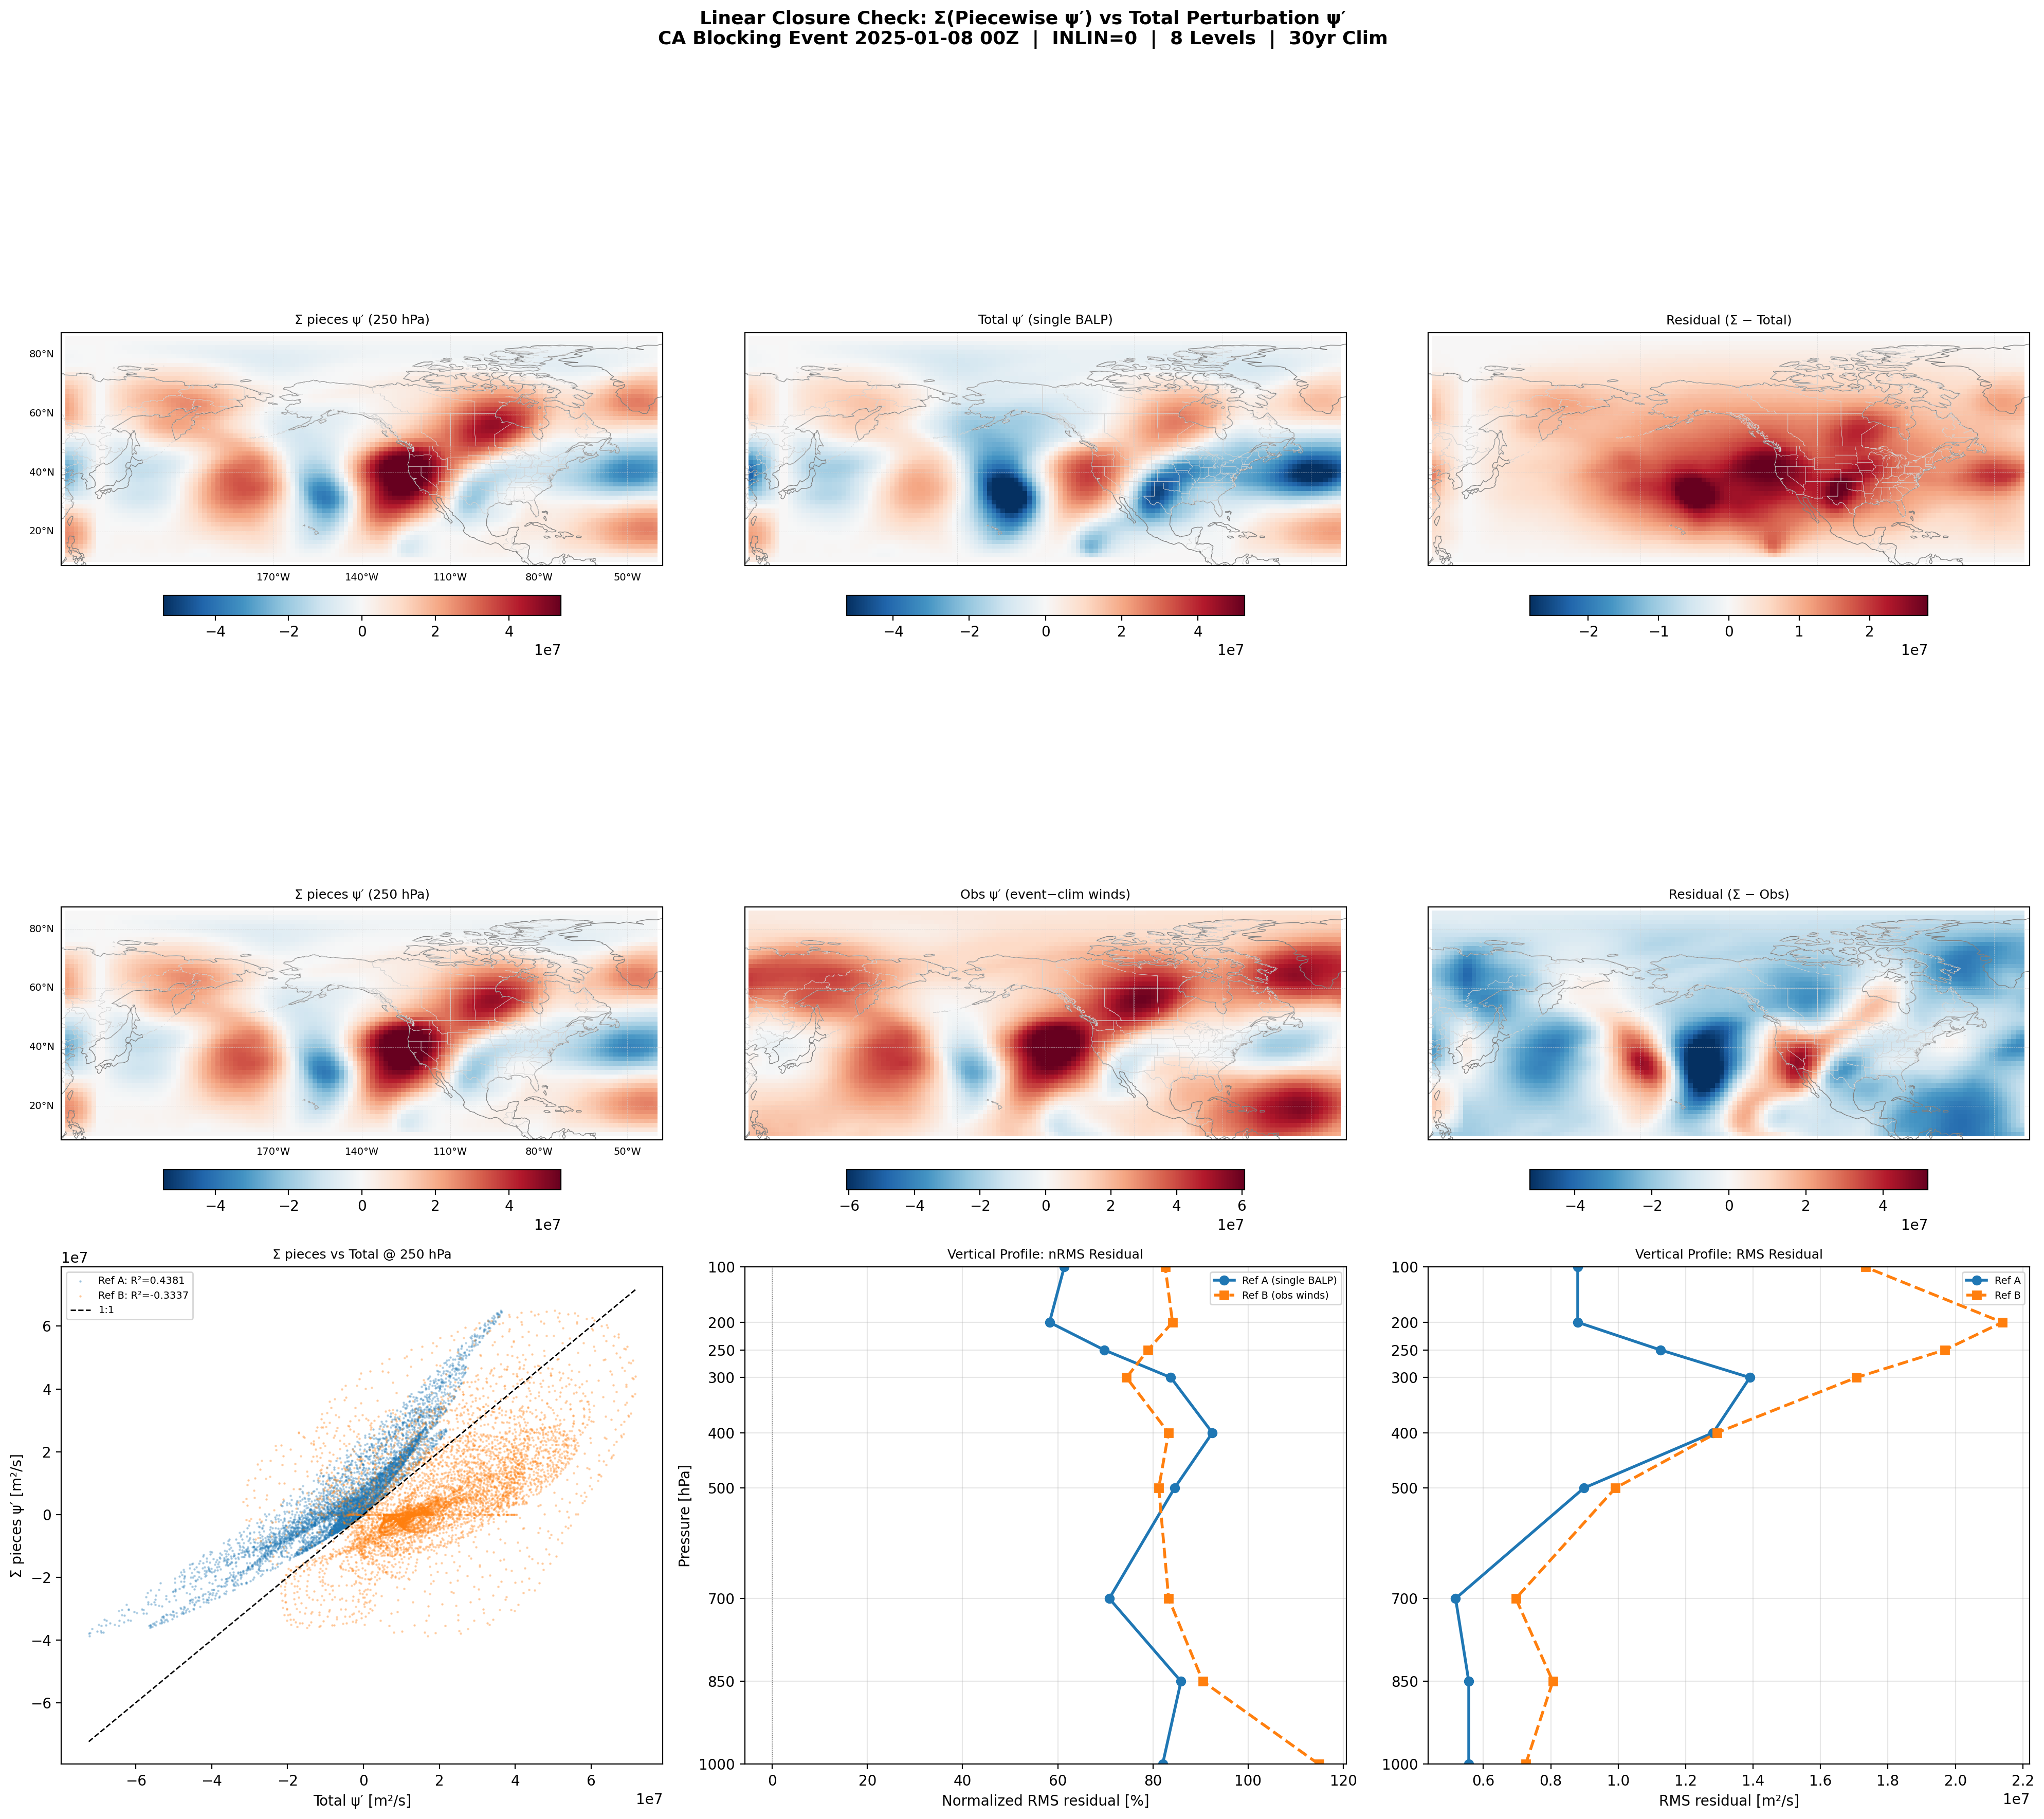
\includegraphics[width=0.95\textwidth]{figs/wu/closure_check.png}
  \caption[Linear closure check]{\textbf{Step 11.} Linear-closure check:
  the sum of the three piecewise $\psi'$ against a single all-levels
  inversion.  On the 9-level (top-100) grid the agreement is moderate
  ($R^2\!\approx\!0.44$ at 250\,hPa) --- a real grid effect, not a solver
  error (\Cref{sec:wu_converge}).}
  \label{fig:wu_closure}
\end{figure}


\part{The Python Spherical-Harmonic Port}
\chapter{Spherical-Harmonic Operators}
\label{chap:sh}

The horizontal operators ($\nabla$, $\Lap$, $\Lapinv$, Helmholtz,
Jacobian) are computed via \textbf{spherical-harmonic} (SH) transforms
delegated to \texttt{pvtend.sh\_ops}.  This chapter documents the
wrappers in \texttt{sh\_ppvi.operators}, in particular how the
hemispheric ERA5 grid is extended to a full sphere by
\emph{parity mirroring}.

\section{Hemispheric Grid and Parity Mirroring}

The working grid is a Northern-Hemisphere lat-lon patch
($10.5^\circ$N--$85.5^\circ$N, $-169.5^\circ$E--$-40.5^\circ$E,
$\Delta\phi=\Delta\lambda=1.5^\circ$).  SH transforms, however,
require a \emph{full sphere}.  The function
\texttt{parity\_mirror(field, lat, kind)} extends a NH field across
the equator with prescribed symmetry:

\begin{itemize}\setlength\itemsep{0pt}
\item \texttt{kind="scalar"}: even reflection,
      $f(-\phi,\lambda)=+f(\phi,\lambda)$ —
      used for $\psi$, $\Phi$, $q$;
\item \texttt{kind="v"} (vector meridional component):
      odd reflection,
      $f(-\phi,\lambda)=-f(\phi,\lambda)$ — used for the RHS of
      divergence-like Poisson problems.
\end{itemize}

\noindent After the spectral operation the SH field is inverse-transformed
back to grid space and restricted to the NH.  This is hidden inside
each wrapper.

\section{Horizontal Operators}

All wrappers act level-by-level on $(K,n_{\text{lat}},n_{\text{lon}})$
arrays.

\paragraph{Gradient.} (\texttt{operators.gradient})
\begin{equation}
\frac{\partial f}{\partial x}=\frac{1}{a\cos\phi}\frac{\partial f}{\partial\lambda},
\qquad
\frac{\partial f}{\partial y}=\frac{1}{a}\frac{\partial f}{\partial\phi}.
\end{equation}

\paragraph{Laplacian.} (\texttt{operators.laplacian})
\begin{equation}
\Lap f = \frac{1}{a^{2}\cos^{2}\phi}\frac{\partial^{2}f}{\partial\lambda^{2}}
       + \frac{1}{a^{2}\cos\phi}\frac{\partial}{\partial\phi}\!
         \left(\cos\phi\,\frac{\partial f}{\partial\phi}\right).
\end{equation}
In spectral space, $\widehat{\Lap f}_{l,m}=-\lambda_l\,\hat f_{l,m}$
with the eigenvalues
\begin{equation}
\lambda_l=\frac{l(l+1)}{a^{2}},\qquad l=0,1,2,\ldots
\label{eq:laplacian_eigs}
\end{equation}

\paragraph{Poisson inversion.} (\texttt{operators.laplacian\_inv})
\begin{equation}
\Lap\chi=\mathrm{rhs}\;\Longrightarrow\;
\hat\chi_{l,m}=
\begin{cases}
  -\hat{\mathrm{rhs}}_{l,m}/\lambda_l, & l\geq 1,\\
  0,                                    & l=0\;\text{(mean-zero gauge)}.
\end{cases}
\label{eq:laplacian_inv}
\end{equation}

\paragraph{Helmholtz decomposition.} (\texttt{operators.helmholtz})
\begin{equation}
(u,v) = \nabla^{\perp}\psi + \nabla\chi
\;\Longleftrightarrow\;
\psi=\Lapinv\zeta,\quad \chi=\Lapinv\delta,
\end{equation}
where $\zeta=\partial v/\partial x-\partial u/\partial y$ and
$\delta=\partial u/\partial x+\partial v/\partial y$.

\paragraph{Jacobian.} (\texttt{operators.jacobian})
\begin{equation}
J(a,b)=\frac{\partial a}{\partial x}\frac{\partial b}{\partial y}
      -\frac{\partial a}{\partial y}\frac{\partial b}{\partial x}.
\end{equation}

\paragraph{$\nabla\!\cdot\!(f\nabla\psi)$.} (\texttt{operators.div\_f\_grad})
Because $f=f(\phi)$ only,
\begin{equation}
\nabla\!\cdot\!(f\nabla\psi)=f\Lap\psi+\beta\,\frac{\partial\psi}{\partial y}.
\end{equation}

\begin{keybox}[Vertical x horizontal separability]
Every horizontal SH operator acts level-by-level; every vertical
operator ($D_1$, $D_2$) acts column-by-column.  The full PPVI operator
\cref{eq:F_op} is therefore a sum of \emph{separable} actions, which
is what makes a level-mean spectral preconditioner of the vertical
operator possible.
\end{keybox}

\chapter{Forward Operator: Ertel PV}
\label{chap:forward}

Two equivalent implementations of Ertel PV exist in
\texttt{sh\_ppvi.forward}:

\section{From $(\psi,\Phi)$ — \texttt{ertel\_q\_sh}}

This is the operator we wish to \emph{invert}.  It is
\cref{eq:Q} verbatim.

\begin{lstlisting}[caption={\texttt{forward.py: ertel\_q\_sh}},label={lst:ertel_q_sh}]
def ertel_q_sh(psi, Phi, lat, lon):
    """Q = g * (lap psi + f) * (kappa*pi/(p*cp)) * d^2 Phi/d pi^2 * 1e6
    Returns PV in PVU (10^-6 K m^2 / kg s)."""
    zeta  = laplacian(psi, lat, lon)                       # 1/s
    f     = coriolis(lat)[None, :, None]                   # 1/s
    D2Phi = d_pi_pi(Phi)                                   # m^2/s^2
    coeff = (KAPPA * PI_VALS / (PLEVS_PA * CP))[:, None, None]
    return G * (zeta + f) * coeff * D2Phi * 1.0e6
\end{lstlisting}

\section{From ERA5 primitives — \texttt{ertel\_q\_from\_uv}}

A second implementation uses ERA5 winds and temperature directly:
\begin{equation}
Q=-g\,(\zeta+f)\,\frac{\partial\theta}{\partial p}\times 10^{6}\;[\PVU],
\end{equation}
with $\partial\theta/\partial p$ from \texttt{np.gradient} on the
non-uniform pressure grid.  This serves as a \emph{reference}
diagnostic when validating the closure between $\bpsi,\bPhi,\theta$.

\begin{warnbox}[Why both?]
The two formulas differ only by the choice of which hydrostatic
relation closes them.  \texttt{ertel\_q\_sh} uses
$\partial\Phi/\partial\pi=-c_p\theta$ and SH vorticity from $\psi$;
\texttt{ertel\_q\_from\_uv} uses direct $\partial\theta/\partial p$
and SH vorticity from $(u,v)$.  For a perfectly balanced state the
two are identical.  The \emph{difference} between them is a useful
balance diagnostic (compare the Wu\,vs.\,ERA5 PV check of
\Cref{chap:wu_pipeline}).
\end{warnbox}

\chapter{The Wu Non-Dimensional BALNC Port (Spherical Harmonics)}
\label{chap:wu_balnc}

This chapter documents the \emph{second}, independent inversion thread
in the repository: a faithful spherical-harmonic (SH) re-implementation
of W.~Wu's finite-difference total-PV inversion code
\texttt{qinvert21\_94.f} (the Fortran reference of
\Cref{chap:wu_solver,chap:wu_pipeline}).  Unlike the $\psi$--$\Phi$
Charney/$f_0$-plane closures of \Cref{sec:closure}, this thread
works in Wu's own \textbf{non-dimensional units} and inverts the coupled
\emph{H-equation} (geopotential-like) and \emph{$\psi$-equation}
(streamfunction) system by outer Picard iteration.  The code lives in
\texttt{sh/sh\_ppvi/} (\texttt{nondim.py}, \texttt{sor.py},
\texttt{coords.py}, \texttt{wu\_ops.py}, \texttt{balnc.py},
\texttt{balp.py}) and the SH operators it calls live in
\texttt{pvtend.sh\_ops}.

\begin{keybox}[Status at time of writing]
The \textbf{BALNC} (full balanced) Pass~C \emph{does not yet converge}.
With all nonlinear terms frozen and under-relaxation
$\mathrm{part}=0.05$, the streamfunction norm grows monotonically
($|\psi|\!:64\!\to\!381$ over 200 outer iterations) rather than
settling; with $\mathrm{part}=0.3$ it diverges explosively
($|\psi|\!\to\!\mathrm{NaN}$ by iteration~100).  The cause is a residual
$H$--$\psi$ feedback, \emph{not} the Helmholtz conditioning hypothesised
in earlier notes (see \Cref{sec:wu_open}).
\end{keybox}

\section{Wu Non-Dimensionalisation}
\label{sec:wu_nondim}

All quantities are scaled by the constants assembled in
\texttt{nondim.Scales} (mirroring \texttt{qinvert21\_94.f} L213--276).
For the standard $1.5^\circ$ grid ($\Delta\lambda=1.5^\circ$, $N_L=10$
levels):

\begin{center}\small
\begin{tabular}{lll}
  \toprule
  Scale & Definition & Value ($1.5^\circ$, $N_L{=}10$) \\
  \midrule
  $\mathrm{DPI}$        & $500/N_L$                                  & $50$ \\
  $\mathrm{LL}$         & $(2\!\times\!10^{7}/\pi)\cdot\Delta\lambda\cdot\pi/180$ & $1.667\times10^{5}$ m \\
  $\mathrm{FF}$         & reference Coriolis                          & $10^{-4}$ s$^{-1}$ \\
  $\mathrm{THO}$        & $\mathrm{FF}^2\,\mathrm{LL}^2/\mathrm{DPI}$ & $5.556$ K \\
  $\mathrm{FRC}$        & $\mathrm{DPI}\cdot\mathrm{THO}/(\mathrm{FF}^2\mathrm{LL}^2)$ & $\equiv 1$ \\
  $\mathrm{QCONST}$     & $10^{6}\kappa\,g\,c_p\,\mathrm{FF}\,\mathrm{THO}/(p_0\,\mathrm{DPI})$ & $0.313$ PVU \\
  $\mathrm{UC}$         & $\mathrm{DPI}\cdot\mathrm{THO}/(\mathrm{FF}\cdot\mathrm{LL})$ & $16.67$ m\,s$^{-1}$ \\
  $H_{\text{factor}}$   & $g/(\mathrm{THO}\cdot\mathrm{DPI})$         & $3.530\times10^{-2}$ \\
  \bottomrule
\end{tabular}
\end{center}

\noindent The field transforms (\texttt{nondim.py}) are
\begin{align}
H_{\text{nd}} &= \Phi_{\text{phys}}\,/\,(\mathrm{THO}\cdot\mathrm{DPI}),
   &\Phi_{\text{phys}}&=g\,z\ [\text{m}^2\,\text{s}^{-2}], \\
\psi_{\text{nd}} &= \psi_{\text{phys}}\cdot 10^{-5}\cdot H_{\text{factor}},
   &\theta_{\text{nd}}&=\theta_{\text{phys}}/\mathrm{THO}, \\
q_{\text{nd}}(k) &= \mathrm{PIF}(k)\,q_{\text{phys}}(k)\,/\,(10^{2}\,\mathrm{QCONST}),
   &\mathrm{PIF}(k)&=(p_k/p_0)^{2.5\kappa}.
\end{align}

\begin{warnbox}[Two subtle factor-of-$g$ traps]
(1) Wu reads heights in \emph{metres}; our $H_{\text{phys}}$ is a
\emph{geopotential} $\Phi=gz$, so \texttt{nondim\_H} divides by
$(\mathrm{THO}\cdot\mathrm{DPI})$ directly (not by $H_{\text{factor}}=g/(\cdots)$),
otherwise a spurious extra $g$ enters.
(2) The vertical operators \emph{must} be built on Wu's non-dimensional
$\pi$, \texttt{PI\_WU}$=c_p(p/p_0)^\kappa/\mathrm{DPI}$ (with
$\Delta\pi_{\text{wu}}\!\approx\!1$ per level), \emph{not} on the
physical $\pi=(p/p_0)^\kappa$ (with $\Delta\pi\!\approx\!0.05$).  The
latter inflates $BB$ from $\mathcal{O}(-10)$ to $\mathcal{O}(-3886)$ and
blows up the static-stability term \texttt{STB} (\texttt{sor.py}
post-\texttt{build\_BB\_BH\_BL} comment).
\end{warnbox}

\section{Vertical Operator: \texorpdfstring{$BB,BH,BL$}{BB,BH,BL}}
\label{sec:wu_vertical}

Wu's second-$\pi$-derivative stencil (\texttt{sor.build\_BB\_BH\_BL},
mirroring \texttt{qinvert21} L202--209), evaluated on \texttt{PI\_WU}:
\begin{equation}
BB_k = \frac{-2}{(\pi_{k+1}{-}\pi_k)(\pi_k{-}\pi_{k-1})},\quad
BH_k = \frac{2}{(\pi_{k+1}{-}\pi_k)(\pi_{k+1}{-}\pi_{k-1})},\quad
BL_k = \frac{2}{(\pi_{k+1}{-}\pi_{k-1})(\pi_k{-}\pi_{k-1})},
\end{equation}
so that $\partial^2 f/\partial\pi^2|_k \approx BL_k f_{k-1}+BB_k f_k+BH_k f_{k+1}$.
Numerically (interior $k=1\ldots8$):
\begin{center}\small
\begin{tabular}{rrrrr}
\toprule
$k$ & $BB_k$ & $BH_k$ & $BL_k$ & $BB_k{+}BH_k{+}BL_k$ \\
\midrule
1 & $-9.637$ & $4.679$ & $4.958$ & $\sim 0$ \\
2 & $-4.121$ & $1.285$ & $2.836$ & $\sim 0$ \\
3 & $-2.472$ & $1.408$ & $1.064$ & $\sim 0$ \\
4 & $-2.903$ & $1.365$ & $1.539$ & $\sim 0$ \\
5 & $-2.230$ & $1.035$ & $1.195$ & $\sim 0$ \\
6 & $-1.611$ & $0.733$ & $0.878$ & $\sim 0$ \\
7 & $-2.268$ & $1.424$ & $0.844$ & $\sim 0$ \\
8 & $-3.314$ & $1.538$ & $1.776$ & $\sim 0$ \\
\bottomrule
\end{tabular}
\end{center}

\begin{keybox}[Row sums vanish $\Rightarrow$ pure 2nd derivative]
The rows sum to $\mathcal{O}(10^{-15})$: the operator has \emph{no}
zeroth-order (Helmholtz) part of its own.  Every bit of vertical
coupling is off-diagonal ($BH_k H_{k+1}+BL_k H_{k-1}$) and, in the
current solver, is evaluated \textbf{explicitly} (lagged) in both the
$\psi$- and $H$-steps.  Explicit treatment of a stiff vertical operator
is only conditionally stable --- the practical stability limit observed
is $\mathrm{part}\lesssim 0.07$.  This is the structural reason the
outer iteration is so fragile (\Cref{sec:wu_open}).
\end{keybox}

\section{The Coupled BALNC System}
\label{sec:wu_balnc_eqs}

\texttt{balnc.balnc\_sh} solves, by outer Picard iteration, the two
spectral elliptic equations below (Wu non-dim throughout).  The SH
Laplacian is $\nabla^2_{\text{wu}}\equiv\mathrm{LL}^2\nabla^2_{\text{sph}}$
(\texttt{wu\_ops.lap\_wu}), so its eigenvalue at total wavenumber $n$ is
$-n(n{+}1)\,\mathrm{LL}^2/a^2$.

\paragraph{$\psi$-equation (Poisson; \texttt{\_psi\_rhs}).}
\begin{equation}
\nabla^2_{\text{wu}}\psi_k
   = \underbrace{\frac{q_k - f\,\mathrm{STB}_k + \nabla^2_{\text{wu}}H_k
        - \mathrm{ZNL}_k + \mathrm{ZL}_k + \mathrm{ZP}_k}{f+\mathrm{STB}_k}}_{\text{RHS}_\psi},
\label{eq:wu_psi}
\end{equation}
with $\mathrm{STB}_k=BL_kH_{k-1}+BB_kH_k+BH_kH_{k+1}$ (static stability),
floored at $10^{-4}$.

\paragraph{$H$-equation (modified Helmholtz; \texttt{\_H\_rhs}).}
\begin{equation}
\bigl(\nabla^2_{\text{wu}} + \mathrm{ASI}_k\,BB_k\bigr)H_k
  \;+\;\mathrm{ASI}_k\bigl(BH_kH_{k+1}+BL_kH_{k-1}\bigr)
  \;=\;\underbrace{f\,\mathrm{VOR}_k+\mathrm{ZNL}_k+q_k+\mathrm{ZL}_k+\mathrm{ZP}_k}_{rh_k},
\label{eq:wu_H}
\end{equation}
where $\mathrm{VOR}_k=\nabla^2_{\text{wu}}\psi_k$ and the absolute
isentropic vorticity $\mathrm{ASI}_k=f+\mathrm{VOR}_k$ (floored so
$\mathrm{ASI}\ge 10^{-4}$).  The $H$-step is solved by an
operator-split modified-Helmholtz inversion (\texttt{wu\_ops.inv\_helm\_wu}
$\to$ \texttt{pvtend.sh\_ops.invert\_helmholtz\_sh}):
\begin{equation}
c_k=\overline{\mathrm{ASI}_k}\,BB_k\ \ (\text{constant shift}),\qquad
\text{remainder }(\mathrm{ASI}_k-\overline{\mathrm{ASI}_k})BB_kH_k\ \text{lagged explicitly.}
\end{equation}

\paragraph{Cross-isobaric / nonlinear terms (\texttt{\_zl\_zp}, \texttt{\_znl}).}
\begin{align}
\mathrm{ZL}_k &= \frac{1}{\cos^2\phi}\,
   \Bigl(\tfrac{\partial H_x}{\partial\pi}\Bigr)_k
   \Bigl(\tfrac{\partial\psi_x}{\partial\pi}\Bigr)_k, &
\mathrm{ZP}_k &= \Bigl(\tfrac{\partial H_y}{\partial\pi}\Bigr)_k
   \Bigl(\tfrac{\partial\psi_y}{\partial\pi}\Bigr)_k, \\
\mathrm{ZNL}_k &= 2\,J(\psi_x,\psi_y)_k + \beta\,\psi_{y,k}.
\end{align}
$\mathrm{ZL}$ is \emph{bilinear} in $H$ and $\psi$; $\mathrm{ZNL}$ is
\emph{quadratic} in $\psi$.  As $\psi$ grows during Picard these terms
amplify $\text{RHS}_\psi$ and feed divergence, so the current code
\textbf{freezes} $\mathrm{ZL},\mathrm{ZP},\mathrm{ZNL}$ at the initial
(event-state) field (\texttt{balnc.py} ``freeze block'').

\section{SH Realisation of the Wu Operators}
\label{sec:wu_sh_ops}

\begin{center}\small
\begin{tabular}{lll}
\toprule
Wu non-dim operator & SH backend (\texttt{pvtend.sh\_ops}) & Notes \\
\midrule
$\mathrm{LL}^2\nabla^2$ (\texttt{lap\_wu})       & \texttt{laplacian\_sh}        & eigval $-n(n{+}1)/a^2$ \\
$(\mathrm{LL}^2\nabla^2)^{-1}$ (\texttt{inv\_lap\_wu}) & \texttt{invert\_laplacian\_sh} & $n{=}0$ pinned to 0 \\
$(\mathrm{LL}^2\nabla^2{+}c)^{-1}$ (\texttt{inv\_helm\_wu}) & \texttt{invert\_helmholtz\_sh}$^\dagger$ & $c_{\text{sh}}{=}c/\mathrm{LL}^2$ \\
$\mathrm{LL}\,\nabla$ (\texttt{grad\_wu})        & \texttt{gradient\_sh}         & \\
Jacobian (\texttt{jac\_wu})                      & \texttt{gradient\_sh}$\times$2 & \\
$n<2$ projector (\texttt{filter\_low\_modes\_sh})$^\dagger$ & --- & m-major packing \\
\bottomrule
\end{tabular}
\end{center}
\noindent$^\dagger$ \texttt{invert\_helmholtz\_sh} and
\texttt{filter\_low\_modes\_sh} were \textbf{added} to
\texttt{pvtend.sh\_ops} for this thread.  They are \emph{purely
additive} (new functions + two new \texttt{\_\_all\_\_} entries); no
existing \texttt{sh\_ops} routine was modified, so all prior callers are
unaffected.

\section{Discrepancies between the Wu FD Reference and the SH Port}
\label{sec:wu_discrepancies}

\begin{enumerate}[leftmargin=1.4em]
\item \textbf{Domain / boundary conditions.}  Wu's FD solver works on a
  \emph{bounded NH window} and pins the lateral rows/columns
  ($I{=}1,I{=}N_Y,J{=}1,J{=}N_X$) as Dirichlet walls, which suppresses
  planetary $n\!\le\!1$ modes.  The SH port works on the \emph{hemisphere}
  ($0$--$90^\circ$N, 61 latitudes at $1.5^\circ$) with a parity mirror to
  the full sphere; it has \emph{no} lateral walls.  The inverse Laplacian
  therefore amplifies $n{=}1$ by $a^2/[n(n{+}1)\mathrm{LL}^2]\approx 730\times$.
  \emph{Mitigation:} \texttt{filter\_low\_modes\_sh($n_{\min}{=}2$)}
  projects out $n{=}0,1$ from $\text{RHS}_\psi$ before inversion and
  re-anchors the $n{=}0,1$ content to the initial $\psi$.

\item \textbf{Helmholtz conditioning is \emph{not} the problem.}  Because
  the grid is NH-only ($0$--$90^\circ$N), the hemispheric mean
  $\overline{f}=0.925$ (\emph{not} $0$, as an earlier global-symmetric
  assumption suggested).  Hence
  $c_k=\overline{\mathrm{ASI}_k}\,BB_k$ ranges from $-9.6$ ($k{=}1$) to
  $-3.3$ ($k{=}8$), and the Helmholtz eigenvalues $-n(n{+}1)\mathrm{LL}^2/a^2+c_k$
  stay safely negative and $\mathcal{O}(-10\ldots -3)$ for \emph{all} $n$.
  The $H$-step inversion is well-posed; the previously documented
  ``$c_k\approx 0$'' root cause is \textbf{retracted}.

\item \textbf{Equatorial denominator.}  $\text{RHS}_\psi$ divides by
  $f+\mathrm{STB}$.  On the global sphere $f\!\to\!0$ near the equator
  makes this denominator $\mathcal{O}(0.03)$ and injects spurious
  large-scale content.  \emph{Mitigation:} \texttt{\_psi\_rhs} zeroes the
  RHS wherever $f+\mathrm{STB}<0.3$ (roughly $|\phi|\lesssim 15^\circ$),
  outside Wu's NH analysis window.

\item \textbf{Explicit vertical coupling.}  Wu's FD solver advances the
  vertical $BB/BH/BL$ coupling inside a tridiagonal/SOR sweep; the SH
  port treats the off-diagonal $BH/BL$ terms \emph{explicitly} (lagged).
  This is the dominant stability bottleneck ($\mathrm{part}\lesssim0.07$).

\item \textbf{$f_0$-plane amplitude bias.}  The piecewise closures still
  use $\delta\Phi\approx f_0\delta\psi$ (\Cref{sec:closure}), which
  under-estimates upper-level geopotential and contributes the
  $\sim\!0.1\times$ amplitude bias relative to the Wu Fortran reference.
\end{enumerate}

\section{Open Issues / Not Yet Done}
\label{sec:wu_open}

\begin{warnbox}[The real BALNC non-convergence]
With $\mathrm{ZL/ZP/ZNL}$ frozen and $\mathrm{part}=0.05$, the
$\psi$-\emph{target} \texttt{psi\_new} itself grows
($\,|\text{psi\_new}|:185\!\to\!455$ over 200 iters) while $|H|$ barely
moves ($442\!\to\!452$).  The growth is a slow $H$--$\psi$ feedback:
$\psi\!\uparrow\,\Rightarrow\,\mathrm{VOR}\!\uparrow\,\Rightarrow\,rh_H\!\uparrow\,\Rightarrow\,H$
drifts $\Rightarrow$ $\mathrm{STB},\nabla^2H$ in
$\text{RHS}_\psi$ change $\Rightarrow$ \texttt{psi\_new}$\,\uparrow$.
Freezing the explicit nonlinear terms removed the \emph{fast} Picard
blow-up but not this \emph{slow} linear feedback.
\end{warnbox}

\noindent Concrete TODO items (carried in session findings):
\begin{itemize}[leftmargin=1.4em]
\item \textbf{BALNC convergence (Pass~C).}  Candidate fixes not yet
  tried: (i) solve the $H$--$\psi$ system \emph{coupled} (eliminate
  $\psi$ analytically into the $H$-equation rather than alternating);
  (ii) implicit vertical coupling (tridiagonal solve in $k$ at each
  spectral coefficient) instead of explicit lagging; (iii) relax $H$ at
  iteration~0 as well (currently the first $H$ update is un-relaxed and
  jumps \texttt{psi\_new} from $92$ to $185$).
\item \textbf{Pass~D} (piecewise pieces from the balanced full field,
  \texttt{balp.py}) is \emph{not run} pending a converged Pass~C; and the
  same $n{=}0,1$ projection fix must be inlined into \texttt{balp.py}.
\item \textbf{Filename mismatch:} \texttt{event\_pieces.nc} vs.\
  \texttt{piecewise.nc} between the writer and \texttt{fig8.py} /
  \texttt{make\_figs.py}.
\item \textbf{Validation:} no quantitative comparison of the SH BALNC
  output against the Wu Fortran reference has been performed yet
  (blocked on convergence).
\end{itemize}

\chapter{Conclusions}
\label{chap:conclusion}

\section{Summary}

This handbook documents the \textbf{Wu Fortran piecewise PV inversion
pipeline} \cite{Davis1992} applied to the 2025-01-08 California
blocking event, on a nine-level ERA5 grid with the perturbation split
into a \textbf{surface}, \textbf{lower} and \textbf{upper} piece:

\begin{enumerate}\setlength\itemsep{2pt}
  \item \textbf{Download / climatology / grid} (\texttt{shared\_steps/01--04}) ---
        ERA5 event hour, 30-year mean, and the Fortran \texttt{.grid} inputs.
  \item \textbf{Pass A/B} (\texttt{pvpialln}) --- boundary $\theta$,
        interior Ertel PV (850--200\,hPa), balanced $\psi$, for the mean
        and event states (step~05).
  \item \textbf{Pass C} (\texttt{qinvert21}/BALNC) --- total balanced
        reference (step~06).
  \item \textbf{Pass D} (\texttt{qinvertp21}/BALP) --- the three-piece
        perturbation inversion, \texttt{INLIN}=1 so the pieces sum to the
        total (step~07).
  \item \textbf{Diagnostics} --- Wu-vs-ERA5 PV, induced winds, PV
        advection, cross-sections, 3-D structure, closure (steps~08--11).
\end{enumerate}

\section{Key Findings}

\begin{enumerate}\setlength\itemsep{3pt}

  \item \textbf{Surface heating is a boundary condition, not interior
        PV.}  Interior Ertel PV exists only at $K{=}2..N_L{-}1$
        (850--200\,hPa); the surface (1000) and top (100) levels carry
        the boundary $\theta$.  By Bretherton's equivalence the warm
        surface $\theta'$ is a positive PV \emph{sheet} at the boundary,
        applied as an inhomogeneous Neumann condition.  We invert it as
        its own \textbf{surface piece} (\texttt{QLV}=$\{1\}$), isolating
        the surface thermal forcing.

  \item \textbf{The surface-piece $\psi'$ is predominantly cyclonic for
        this event} ($\sim$84\% of points have $\psi'<0$ at 1000\,hPa),
        because the domain-mean surface $\theta'$ is net warm
        ($\approx+1$\,K).  This is case-dependent, not a law: a net-cold
        surface anomaly would give an anticyclonic surface piece.

  \item \textbf{Wu $Q\to$ SI is the exact constant $10^{-8}$} when
        $\kappa=2/7$ (\Cref{chap:wu_coeffs}).  After the raw-$T$ input
        fix, $Q_{\text{Wu}}\times10^{-8}$ matches ERA5 native Ertel PV
        with median ratio $1.00$, $\corr=0.995$.  The former
        ``$\sim$3.5$\times$ residual'' and any empirical scaling are
        retired.

  \item \textbf{The 9-level (top-100) grid closes the piecewise sum
        better} ($R^2\!\approx\!0.44$ at 250\,hPa) than a uniform-top
        8-level (top-200) grid ($R^2\!\approx\!-0.2$).  The non-uniform
        top is accepted because all analysis of interest is at
        $\le 200$\,hPa.

  \item \textbf{Pass D converges (\texttt{INLIN}=1)}; the earlier
        ``\texttt{INLIN}=0 mandatory'' claim is obsolete.  Pass C's
        ``started diverging'' is a benign post-convergence heuristic.
\end{enumerate}

\begin{table}[H]
\centering\small
\caption{SI unit conventions for all pipeline outputs.}
\label{tab:si_units}
\begin{tabular}{lll}
\toprule
Quantity & Symbol & Units \\
\midrule
Streamfunction          & $\psi$          & m$^{2}$\,s$^{-1}$ \\
Geopotential            & $\Phi = gz$     & m$^{2}$\,s$^{-2}$ \\
Ertel PV                & $q$             & K\,m$^{2}$\,kg$^{-1}$\,s$^{-1}$ \\
PV advection tendency   & $-\mathbf{u}\cdot\nabla q$ & K\,m$^{2}$\,kg$^{-1}$\,s$^{-2}$ \\
Induced wind            & $u,v$           & m\,s$^{-1}$ \\
Pressure                & $p$             & hPa \\
\bottomrule
\end{tabular}
\end{table}

\section{Limitations and Future Work}

\begin{itemize}\setlength\itemsep{2pt}
  \item \textbf{Flat lower boundary.}  The solver treats 1000\,hPa as a
        rigid lid everywhere and ignores topography; over the western-US
        land surface the true lower boundary is well above 1000\,hPa.  A
        terrain-following / surface-pressure lower boundary
        ($p=\mathrm{hyam}\,p_0+\mathrm{hybm}\,p_s$) with the actual
        near-surface $\theta$ would be the principal physical upgrade.
        The boundary-$\theta$ Neumann condition itself is standard and
        correct; the GFDL/CSU PPVI tool uses the identical scheme (plus a
        regional ``surgery'' mask of the boundary $\theta$).
  \item \textbf{Coarse vertical/horizontal resolution} ($1.5^\circ$,
        9 levels) limits the static-stability estimate and the closure.
\end{itemize}

%

\appendix
\chapter{Notation Glossary}
\label{app:notation}

\begin{longtable}{lll}
  \toprule
  Symbol & Units & Description \\
  \midrule\endhead
  $a$                  & m            & Earth radius $6.371\times 10^{6}$ \\
  $\alpha$             & --           & Picard under-relaxation parameter \\
  $\beta=2\Omega\cos\phi/a$ & s$^{-1}$\,m$^{-1}$ & meridional grad.\ of $f$ \\
  $\bPhi$              & m$^2$/s$^2$  & climatological mean geopotential \\
  $\bpsi$              & m$^2$/s      & climatological mean streamfunction \\
  $\bq$                & PVU          & climatological mean Ertel PV \\
  $\bzeta=\Lap\bpsi$   & s$^{-1}$     & mean relative vorticity \\
  $c_p$                & J/kg/K       & specific heat at const.\ pressure (1004) \\
  $\dPhi=\Phi-\bPhi$   & m$^2$/s$^2$  & geopotential anomaly \\
  $\dpsi=\psi-\bpsi$   & m$^2$/s      & streamfunction anomaly \\
  $\dq=q-\bq$          & PVU          & Ertel PV anomaly \\
  $D_1,\,D_2$          & --           & 1st/2nd derivative matrices in $\pi$ \\
  $f=2\Omega\sin\phi$  & s$^{-1}$     & Coriolis parameter \\
  $f_0=f(45^\circ)$    & s$^{-1}$     & reference Coriolis \\
  $g$                  & m/s$^2$      & gravity (9.80665) \\
  $J(a,b)$             & varies       & Jacobian \\
  $\kappa=R_d/c_p$     & --           & 0.28586 \\
  $\Lap,\;\Lapinv$     & m$^{-2}$     & spherical Laplacian and its inverse \\
  $\lambda_l=l(l+1)/a^2$ & m$^{-2}$   & SH Laplacian eigenvalue \\
  $\Omega$             & rad/s        & Earth rotation rate $7.292\times10^{-5}$ \\
  $\pi=(p/p_0)^{\kappa}$ & --         & Exner pressure \\
  $p_0$                & Pa           & reference pressure $10^{5}$ \\
  $\phi,\,\lambda$     & rad          & latitude, longitude \\
  $\psi,\,\Phi$        & m$^2$/s,\,m$^2$/s$^2$ & streamfunction, geopotential \\
  PVU                  & $10^{-6}$\,K\,m$^2$/kg/s & potential vorticity unit \\
  $Q,\,q$              & PVU          & Ertel potential vorticity \\
  $\theta=T(p_0/p)^{\kappa}$ & K      & potential temperature \\
  $\zeta=\Lap\psi$     & s$^{-1}$     & relative vorticity \\
  \bottomrule
\end{longtable}

\chapter{Public-API Reference}
\label{app:api}

\section{Part I --- Wu Fortran reference (\texttt{wu/})}

\subsection{\texttt{config.py} (shared)}
\begin{itemize}\setlength\itemsep{0pt}
\item Grid: \texttt{NX=87}, \texttt{NY=51}, \texttt{NW=10};
      \texttt{PLEVS} (10 levels, $1000$--$200$\,hPa).
\item Solver params: \texttt{OMEGS}, \texttt{OMEGH}, \texttt{PART},
      \texttt{INLIN}, \texttt{MAXT}, \texttt{THRSH}, piece definitions.
\item Paths: \texttt{WU\_IN\_DIR}, \texttt{WU\_OUT\_DIR},
      \texttt{FORT\_DIR}, \texttt{FIG\_DIR}.
\end{itemize}

\subsection{Fortran programs (\texttt{wu/fortran/})}
\begin{itemize}\setlength\itemsep{0pt}
\item \texttt{pvpialln\_94UV.f} --- Pass A/B: Ertel PV + balanced
      $\psi,\Phi$ (\Cref{sec:wu_passes}).
\item \texttt{qinvert21\_94.f} (BALNC) --- Pass C: total balanced
      inversion (\cref{eq:wu_psi,eq:wu_H}).
\item \texttt{qinvertp21\_94.f} (BALP) --- Pass D: 3-piece perturbation
      inversion.
\end{itemize}

\subsection{Step drivers (\texttt{wu/steps/})}
\begin{itemize}\setlength\itemsep{0pt}
\item \texttt{05\_wu\_pass\_ab/} --- compile + Pass A/B; writes
      \texttt{meanq}, \texttt{meanh}, \texttt{event\_\{q,h\}.out}.
\item \texttt{06\_wu\_pass\_c/} --- Pass C; writes
      \texttt{event\_bal.out}.
\item \texttt{07\_wu\_pass\_d/} --- Pass D; writes
      \texttt{event\_pert.out}.
\item \texttt{08\_parse\_outputs/} --- ERA5 Ertel PV
      (\cref{eq:wu_ertel_pv}) + Wu/ERA5 comparison.
\item \texttt{09\_pv\_advection/} --- PV advection by induced winds
      (\cref{eq:wu_pvadv}); writes \texttt{pv\_advection.nc}.
\item \texttt{10\_fig8/} --- Davis 2022 Fig.~8 replica
      (\texttt{fig8\_replica.\{png,pdf\}}).
\end{itemize}

\section{Part II --- Wu Python finite-difference port (\texttt{wu\_python/})}

\subsection{\texttt{wu\_python/core/grid.py}}
\begin{itemize}\setlength\itemsep{0pt}
\item \texttt{FC} --- Coriolis $f$ (NY,), \texttt{A} --- 5-pt Laplacian coeffs (NY,5)
\item \texttt{AP} --- $\cos\phi$ (NY,), \texttt{DP/DL} --- grid spacings [m]
\item \texttt{LON2D, LAT2D} --- 2-D meshgrid for plotting
\end{itemize}

\subsection{\texttt{wu\_python/core/nondim.py}}
\begin{itemize}\setlength\itemsep{0pt}
\item Non-dimensional constants: \texttt{G, CP, P0, KAP, DPI, FF, THO, LL}
\item \texttt{PI\_WU} --- Wu-scaled Exner function $\Pi_\text{Wu}=C_p(p/p_0)^\kappa/\text{DPI}$
\item \texttt{BB, BH, BL} --- vertical tridiagonal coefficients (built from PI\_WU)
\end{itemize}

\subsection{\texttt{wu\_python/core/fd\_ops.py}}
\begin{itemize}\setlength\itemsep{0pt}
\item \texttt{laplacian\_5pt(psi)} --- 5-point FD Laplacian (\ref{eq:laplacian_5pt})
\item \texttt{relative\_vorticity(U, V)} --- $\zeta = \partial_x v - \partial_y u$
\end{itemize}

\subsection{\texttt{wu\_python/core/sor\_solver.py}}
\begin{itemize}\setlength\itemsep{0pt}
\item \texttt{sor\_poisson\_2d(rhs, bc, omega, max\_iter, tol)} ---
      Red-black SOR for $\nabla^2\psi=\zeta$ (\ref{eq:sor_update})
\item Numba-accelerated with \texttt{parallel=True}, thread-safe per-row error reduction
\end{itemize}

\subsection{\texttt{wu\_python/core/pv\_calc.py}}
\begin{itemize}\setlength\itemsep{0pt}
\item \texttt{compute\_ertel\_pv(U, V, TH, H, FC)} --- Ertel PV on $\sigma$-levels (\ref{eq:ertel_sigma})
\item \texttt{invert\_vorticity\_balanced(VOR, H, U, V)} --- $\nabla^2\psi=\zeta$ with wind-integrated BC (\ref{eq:psi_boundary})
\item \texttt{\_boundary\_psi\_from\_winds(H, U, V)} --- Davis eq.~2.40 boundary integration
\end{itemize}

\subsection{\texttt{wu\_python/core/balance.py} (BALNC)}
\begin{itemize}\setlength\itemsep{0pt}
\item \texttt{balnc\_total(Q, H\_init, PSI\_init, THA\_K, ...)} ---
      Coupled $\psi$--$H$ SOR total-balance inversion (Pass~C)
\item \texttt{\_nondim(H, PSI, Q)} --- non-dimensionalization:
      $H_\text{nd}=H/\text{HND}$, $\psi_\text{nd}=\psi/(10^5\cdot\text{HND})$,
      $q_\text{nd}=\text{PIF}_k\cdot q/(10^2\cdot\text{QCONST})$
\item \texttt{\_h\_solve\_column\_parallel} (in \texttt{balance\_parallel.py}) ---
      Implicit vertical tridiagonal Thomas solver per column, numba \texttt{prange} over $j$
\end{itemize}

\subsection{\texttt{wu\_python/core/piecewise.py} (BALP)}
\begin{itemize}\setlength\itemsep{0pt}
\item \texttt{balp\_pieces(Q\_event, Q\_mean, PSI\_mean, H\_mean, ...)} ---
      Piecewise perturbation inversion (Pass~D)
\item Exact 1:1 port of \texttt{qinvertp21\_94.f} subroutine BALP
\item \texttt{\_compute\_mean\_coeffs(HB\_nd, SBR\_nd)} --- pre-compute
      SLL, SPP, AVO, STB, ASI, BSI, APHI from non-dimensional mean state
\item \texttt{\_balp\_solve(SP, HP, QP, TP, coeffs, ...)} --- core BALP
      solver: $\psi'$ SOR (numba 2-D per level) + $H'$ SOR (3-D pointwise)
\end{itemize}

\subsection{\texttt{wu\_python/config.py}}
\begin{itemize}\setlength\itemsep{0pt}
\item Solver params: \texttt{OMEGS, OMEGH, PART, THRSH, MAXT, MAX\_ITER}
\item Parallelism: \texttt{N\_WORKERS=32} (ProcessPoolExecutor),
      \texttt{NUM\_CORES=64} (numba threads)
\item Piece definitions: \texttt{PIECES} (lower/middle/upper)
\end{itemize}

\subsection{Step drivers (\texttt{wu\_python/steps/})}
\begin{itemize}\setlength\itemsep{0pt}
\item \texttt{05\_pass\_ab/run\_pass\_ab.py} --- Pass A/B: Ertel PV + $\psi$
\item \texttt{06\_pass\_c/run\_pass\_c.py} --- Pass C: total balanced inversion
\item \texttt{07\_pass\_d/run\_pass\_d.py} --- Pass D: 3-piece perturbation (ProcessPoolExecutor)
\item \texttt{08\_parse\_outputs/parse\_and\_pv.py} --- ERA5 vs Wu PV comparison
\item \texttt{09\_pv\_advection/pv\_advection.py} --- PV advection by induced winds
\item \texttt{10\_fig8/fig8\_replica.py} --- Davis 2022 Fig.~8 replica
\end{itemize}

\section{Shared utilities (\texttt{pvtend.sh\_ops})}

All operate level-by-level on a NH grid via internal parity-mirroring.
Retained for reference; the Wu Python track uses finite differences instead.
\begin{itemize}\setlength\itemsep{0pt}
\item \texttt{invert\_helmholtz\_sh}$^\dagger$,
      \texttt{filter\_low\_modes\_sh}$^\dagger$ --- added for the earlier
      SH BALNC port; purely additive, backward-compatible.
\end{itemize}
\noindent$^\dagger$ new functions; no existing \texttt{sh\_ops} routine
was modified.



\bibliographystyle{plain}
\bibliography{refs}

\end{document}
